\chapter{Implementation}
\label{cap:implementacion}

This chapter reports the experimental work. It begins with process discovery and conformance checking of the event log with four tools, which validate the event log and the reference model and reveal the finding that conditions the predictive design. It then describes the PPM experimental design: the experiments and their nomenclature, the prefixes and their cutting rules, the encodings, the split, the models and the metrics. Next, it presents the results of the three predictions carried out: next-activity prediction, ICU admission without planning information and prolonged length of stay. It then presents the complementary analyses and, finally, a comparative synthesis and the contrast with the Entropy-Driven Next Activity Prediction Approach of Zare et al.\ \cite{zare2025}.

\section{Process Discovery and Conformance Checking}
\label{sec:discovery}

Before training any predictive model, the event log was analyzed with the PM techniques of Section~\ref{sec:pm}, with two aims: to validate the event log and the reference model, and to understand the process as it is recorded in the data. The work was carried out with four tools: ProM\footnote{\url{https://promtools.org/}}, Disco\footnote{\url{https://fluxicon.com/disco/}}, Celonis\footnote{\url{https://www.celonis.com/}} and PM4Py\footnote{\url{https://processintelligence.solutions/pm4py}}. This section is organized in four parts. Section~\ref{sec:cuatro_herramientas} describes the loading of the event log in the four tools and the reading of the discovered process with the visual tools, Disco and Celonis. Section~\ref{sec:descubiertos} applies two discovery algorithms, the Heuristics Miner and the Inductive Miner, in ProM and PM4Py, to see which one produces the best model of the event log. Section~\ref{sec:conformance} checks the event log against the reference model of Section~\ref{sec:modelo}. Section~\ref{sec:aporte_discovery} collects what this analysis contributes to the predictive design.

\subsection{The Event Log in the Four Tools}
\label{sec:cuatro_herramientas}

The XES file of the event log was loaded into ProM, Disco, Celonis and PM4Py. The four tools read 1,475 cases, 7,780 events and 14 activities; Disco and PM4Py also agree on 97 variants and 59 arcs of the DFG, and on a median case duration of 3.2 days (mean 4.9). This agreement validates the event log as a common input and rules out formatting errors or misinterpretation of the timestamps. The two visual tools give the first reading of the process. The frequency map of Disco (Figure~\ref{fig:disco}, in Chapter~\ref{cap:datos}) shows the dominant path through the operating theater and the ward destination, and the secondary paths through the consultations, the post-anesthesia care unit and the ICU. The Process Explorer of Celonis (Figure~\ref{fig:celonis}) shows the same 14 activities with their case frequencies and allows filtering the cases by variant, which was used to inspect the atypical trajectories one by one.

\begin{figure}[htbp]
\centering
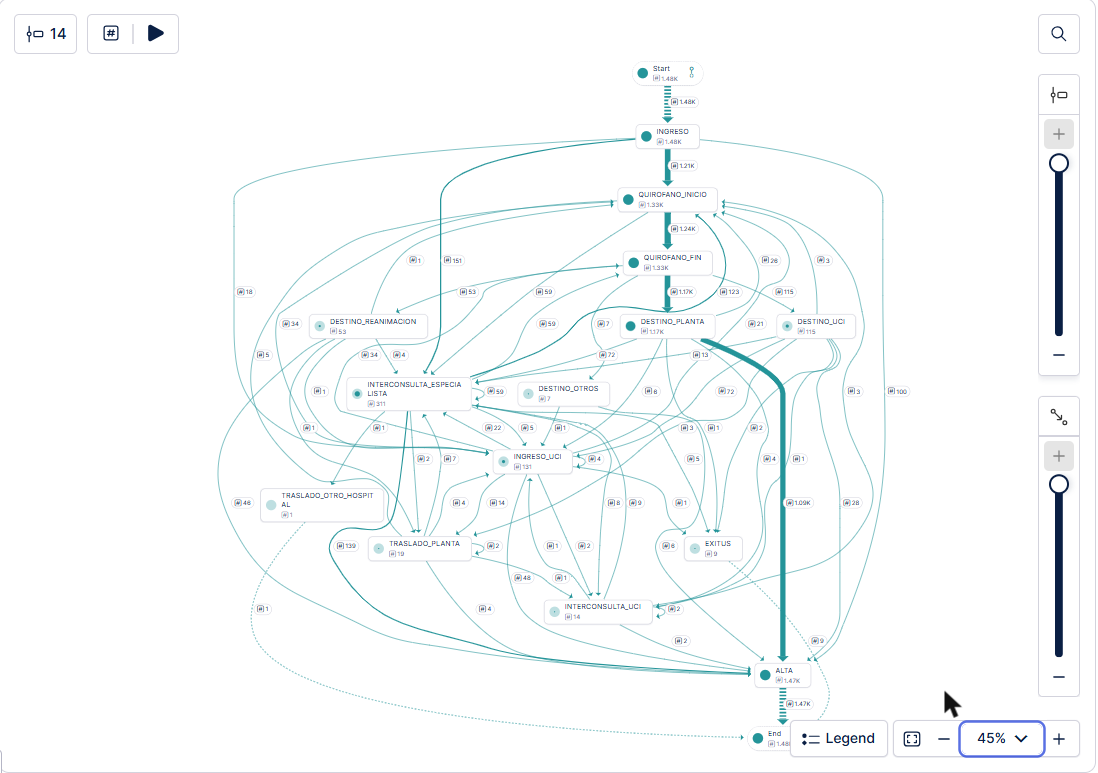
\includegraphics[width=0.9\textwidth]{celonis_explorer}
\caption{Process Explorer of Celonis with the 14 activities of the event log.}
\label{fig:celonis}
\end{figure}

\subsection{Discovered Models}
\label{sec:descubiertos}

Two discovery algorithms were applied, each in two tools, ProM and PM4Py, so that the results could be compared between independent implementations. The Heuristics Miner was run with a dependency threshold of 0.9, which keeps only the transitions that appear in a stable way and filters the infrequent ones; the Inductive Miner was run in its infrequent variant with a noise threshold of 0.2, which guarantees a sound model at the cost of generalizing more. These are the two algorithms described in Section~\ref{sec:pm} and the thresholds are the usual starting values of both tools. Their quality was measured with alignments against the complete event log (Table~\ref{tab:discovery}).

\begin{table}[htbp]
\centering
\caption{Quality of the discovered models (alignments against the event log).}
\label{tab:discovery}
\begin{tabular}{lccc}
\toprule
Model & Fitness & Fitting traces & Precision \\
\midrule
Heuristics Miner, dependency 0.9 (PM4Py) & \textbf{0.972} & 89.9\% & \textbf{0.915} \\
Heuristics Miner (iDHM), dependency 0.9 (ProM) & \textbf{0.984} & -- & -- \\
Inductive Miner infrequent 0.2 (PM4Py) & 0.917 & 76.1\% & 0.510 \\
Inductive Miner infrequent 0.2 (ProM) & 0.912 & -- & -- \\
\bottomrule
\end{tabular}
\end{table}

The Heuristics Miner (Figure~\ref{fig:heuristics}) is the best discovered model in both tools: it represents three of the four exits of the operating theater (\code{DESTINO\_OTROS}, with seven events, is discarded) and the step \code{DESTINO\_UCI} $\rightarrow$ \code{INGRESO\_UCI}, and discards the infrequent activities. ProM, with its reference implementation, the iDHM (Figure~\ref{fig:prom}), reproduces the result with the same thresholds. The Inductive Miner, on the other hand, loses precision. In 34 ICU admissions the actual transfer has a timestamp earlier than the end of the surgery (21 of them form the variant \code{QUIROFANO\_INICIO} $\rightarrow$ \code{INGRESO\_UCI} $\rightarrow$ \code{QUIROFANO\_FIN} $\rightarrow$ \code{DESTINO\_UCI} $\rightarrow$ \code{ALTA}). To cover that order, the algorithm takes the ICU branch out of the surgical block and makes it concurrent, which admits much more behavior than appears in the event log.

\begin{figure}[htbp]
\centering
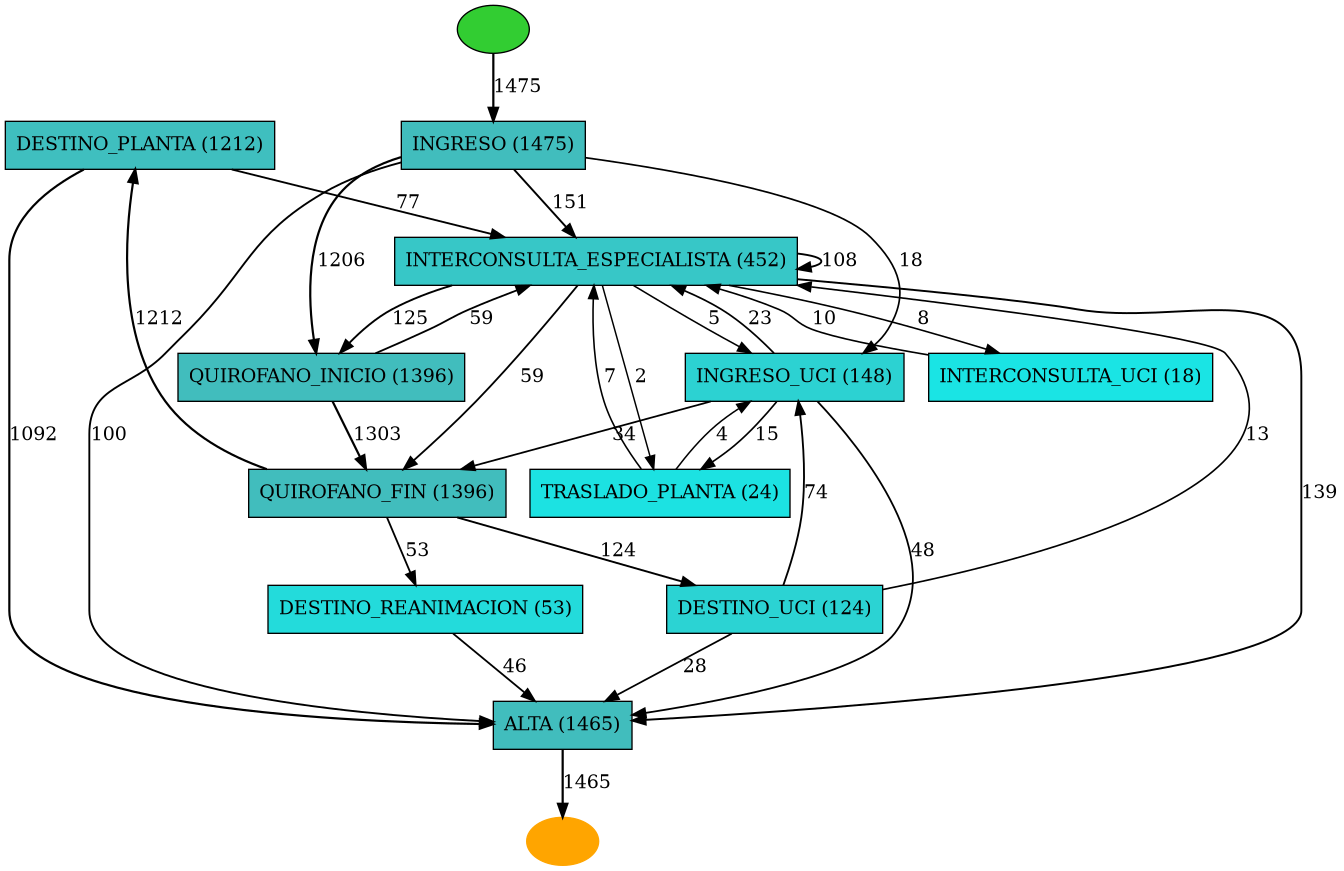
\includegraphics[width=0.9\textwidth]{pm4py_heuristics}
\caption{Heuristic net discovered by PM4Py (dependency 0.9).}
\label{fig:heuristics}
\end{figure}

\begin{figure}[htbp]
\centering
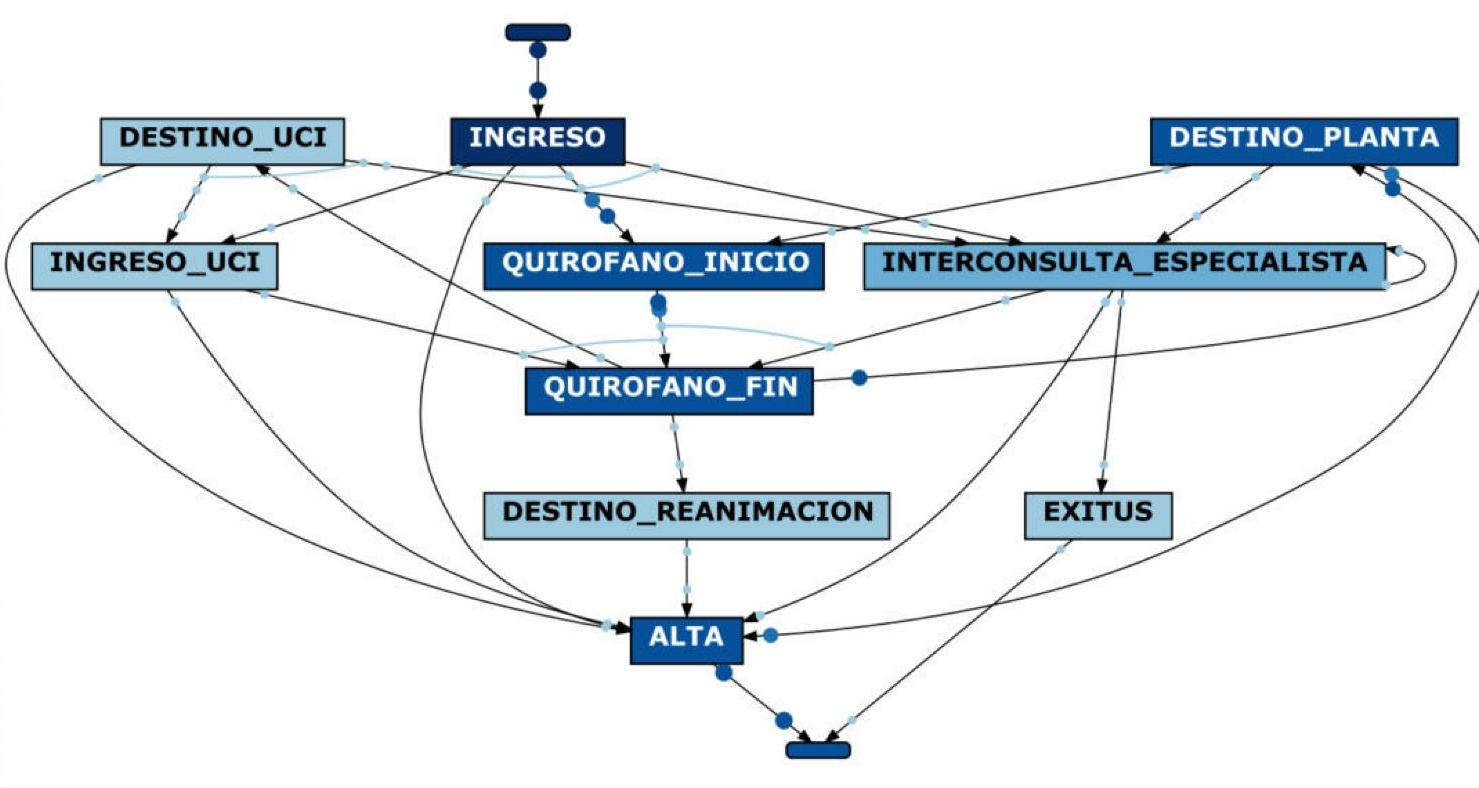
\includegraphics[width=0.9\textwidth]{prom_idhm}
\caption{iDHM in ProM Lite with the same thresholds.}
\label{fig:prom}
\end{figure}

\subsection{Conformance Checking Against the Reference Model}
\label{sec:conformance}

The event log was checked against the reference model of Section~\ref{sec:modelo} (Figure~\ref{fig:bpmn}). For the replay, the tasks of the model were mapped to the activities of the event log as in Table~\ref{tab:actividades}, with one reading imposed by the data (Section~\ref{sec:destino_uci}): the ICU bed reservation of the model corresponds to the ICU destination recorded in the operating theater (\code{DESTINO\_UCI}), which follows the surgery and precedes the ICU admission. The check was made in two tools. In PM4Py, the BPMN model was converted into a Petri net and aligned with the event log: the model reaches a fitness of 0.951 with \textbf{80.9\%} of fitting traces and a precision of 0.639. In the Process Adherence Manager of Celonis, which maps the tasks of the BPMN model to the activities of the event log and counts the cases without deviations, \textbf{80.95\%} of the cases conform (Figure~\ref{fig:celonis_conf}). The agreement between two independent implementations validates the model as the reference of the work.

\begin{figure}[htbp]
\centering
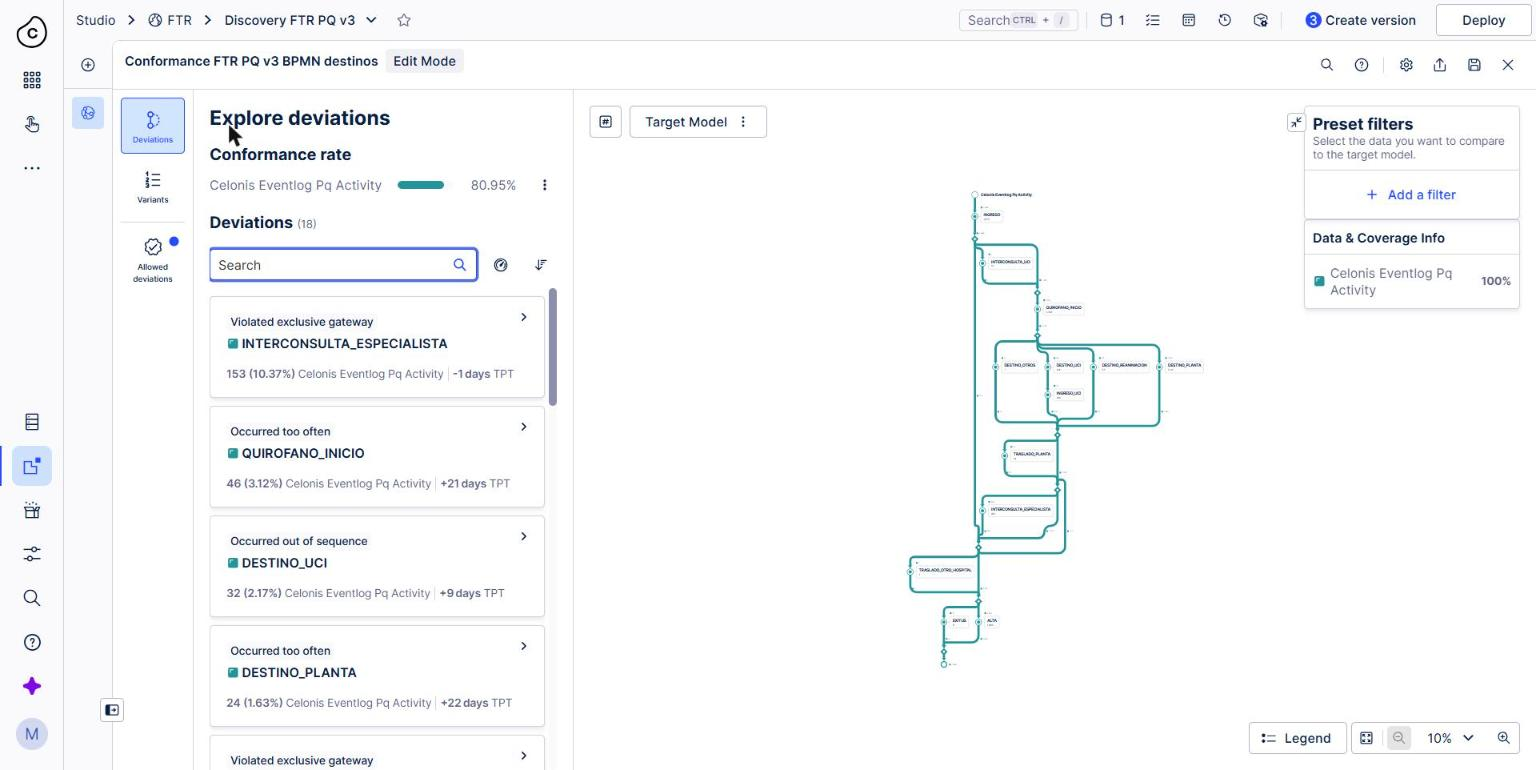
\includegraphics[width=0.85\textwidth]{celonis_conformance}
\caption{Conformance of the event log against the reference BPMN model in the Process Adherence Manager of Celonis (80.95\%).}
\label{fig:celonis_conf}
\end{figure}

The 19\% of cases that do not conform are informative, because their deviations are the behavior that the planned process does not foresee. Three deviations account for most of them.

\begin{itemize}[leftmargin=*]
  \item \textbf{Transfer to the ICU recorded before the destination} (32 cases). Source: the alignments of PM4Py (32 of the 34 transfers of Section~\ref{sec:construccion}; the other two traces are explained by the alignment through another deviation), which report an \code{INGRESO\_UCI} move present in the event log but not allowed by the model at that point. These are the cases of Section~\ref{sec:construccion} in which the ICU bed is occupied while the patient is still in the operating theater, and therefore the actual transfer precedes the end of the surgery and the destination decision.
  \item \textbf{Repeated destinations in reinterventions} (24 cases). Source: the alignments of PM4Py. The model has a single surgery task and a single destination decision, whereas the episodes with two or more interventions record a destination after each one.
  \item \textbf{ICU admission after a ward destination} (20 cases). Source: the Process Adherence Manager of Celonis, which flags it as a violation of the exclusive destination gateway: the case takes the ward branch (\code{DESTINO\_PLANTA}) and then executes \code{INGRESO\_UCI}, which belongs to the ICU branch. The count covers all the interventions of the episode, whereas Table~\ref{tab:destino_uci} considers only the first one, which is why it does not coincide exactly with the 21 unplanned admissions.
\end{itemize}

The third deviation is precisely the unplanned ICU admission: the normative model naturally identifies it as a breach of what was planned.

\subsection{What Discovery Contributes to the Predictive Design}
\label{sec:aporte_discovery}

The findings from the process discovery and conformance checking phases informed the selection of relevant variables, the identification of feasible prediction tasks and the subsequent design of the predictive experiments. Three of them pass directly into the experimental design and are explained below.

First, the postoperative destination ICU anticipates the ICU admission in 100\% of the cases (Table~\ref{tab:destino_uci}). A model that sees \code{DESTINO\_UCI} in the prefix does not predict anything: it reads a decision that the surgical team has already taken and recorded. Its results would measure the consistency of the recording system, not the ability to anticipate a complication. For this reason, the planned destination is removed from the prefixes of Prediction~2, and it is kept only in the complementary analysis B, whose purpose is to measure how much of the admission is decided in the operating theater.

Second, when the planned destination was the ward, the ICU admission arrives with a median of 2.1 days after the operating theater, versus 15 minutes when the ICU was planned. This provides a time horizon in which a prediction would have clinical value: there is time to act between the exit of the operating theater and the deterioration.

Third, the anesthesia recorded at the start of the surgery also reveals the planning. The catalog of anesthesia types of the database distinguishes, within general anesthesia, the values \code{Gral-UCI} and \code{Gral-REA}: general anesthesia for a patient who will be sent to the ICU, or to the post-anesthesia care unit, after the surgery. These values are recorded with \code{QUIROFANO\_INICIO}, that is, before the destination decision, and \code{Gral-UCI} ends in \code{DESTINO\_UCI} in 88 of 122 interventions. The anesthesia therefore anticipates almost the same as the destination and one event earlier. It must be treated in the same way: in Prediction~2 both values are recoded as plain general anesthesia.

\section{Predictive Process Monitoring Experimental Design}

The predictive part of the work follows a single pipeline, summarized in Figure~\ref{fig:pipeline}, which is identical for the three predictions and for the complementary analyses. The event log is cut into prefixes, each prefix is encoded in two ways, the cases are split temporally, the models are trained with three seeds each, and the results are evaluated with metrics suited to each prediction type. The following subsections describe each stage.

The whole experiment is implemented in Python and runs with a single script, \code{run\_final\_v3.py}. The script loads the event table and the case table of the event log, computes the process entropy, builds the prefixes of each prediction with its cutting rule, encodes them, splits the cases temporally, trains the five models with three seeds each and writes the results. It reuses two modules: \code{ppm\_data\_v3.py}, which contains the loading of the event log, the construction of the prefixes, the encodings and the temporal split, and \code{run\_experiments\_v3.py}, which contains the models, the training loop of the neural networks, the metrics and the figures. One complete run of the three predictions takes 551 s on a two-core CPU, without a graphics processing unit, which shows the modest size of the problem. The run leaves in a results folder the metric tables in CSV format, one row per model and seed, the ROC and precision--recall curves, the AUC-ROC per prefix length, the variable importances and an execution log with every figure reported in this chapter. Every table and figure of the chapter can therefore be regenerated from the event log with one command, and the complementary analyses are run with the same modules and different arguments.

\begin{figure}[htbp]
\centering
\begin{tikzpicture}[
  stage/.style={draw=black!60, rounded corners=3pt, fill=black!4, text width=2.38cm, minimum height=3.9cm, align=left, font=\footnotesize, inner sep=5pt, anchor=north},
  num/.style={circle, fill=black!75, text=white, font=\scriptsize\bfseries, minimum size=4.2mm, inner sep=0pt},
  arr/.style={-{Latex[length=2mm]}, thick, black!60}]
\node[stage] (s1) at (0,0) {\hspace*{5.5mm}\textbf{Prefixes}\\[4pt] Trace up to event $k$, $k = 1 \ldots 6$. Never ends in \code{ALTA}, \code{EXITUS} or a transfer to another hospital; cut before the event that defines the label.};
\node[stage, right=0.45cm of s1.north east, anchor=north west] (s2) {\hspace*{5.5mm}\textbf{Encodings}\\[4pt] Aggregate (59--61 variables) for the tree-based models; sequence (embedding + two temporal features + static vector) for LSTM and Transformer.};
\node[stage, right=0.45cm of s2.north east, anchor=north west] (s3) {\hspace*{5.5mm}\textbf{Temporal split}\\[4pt] By admission date, at case level: 64\% training, 16\% validation, 20\% test (the 295 most recent cases).};
\node[stage, right=0.45cm of s3.north east, anchor=north west] (s4) {\hspace*{5.5mm}\textbf{Models}\\[4pt] Five models $\times$ three seeds, basic configuration, no tuning. Threshold chosen on validation (maximum F1-score); early stopping on validation.};
\node[stage, right=0.45cm of s4.north east, anchor=north west] (s5) {\hspace*{5.5mm}\textbf{Metrics}\\[4pt] Outcome: AUC-ROC and AUC per prefix, AUC-PR, Brier, F1-score, recall, precision. Next activity: accuracy and macro F1-score.};
\foreach \i/\n in {s1/1,s2/2,s3/3,s4/4,s5/5} \node[num] at ([xshift=4.2mm,yshift=-4.2mm]\i.north west) {\n};
\foreach \a/\b in {s1/s2,s2/s3,s3/s4,s4/s5} \draw[arr] ([yshift=-1.95cm]\a.north east) -- ([yshift=-1.95cm]\b.north west);
\end{tikzpicture}
\caption{The experimental pipeline, common to the three predictions and to the complementary analyses.}
\label{fig:pipeline}
\end{figure}

\subsection{The Experiments and their Nomenclature}

Six experiments were defined. Three of them are the predictions of the work, named according to the classification of Section~\ref{sec:ppm}: Prediction~1 is a next event prediction (the next activity of the case), and Predictions~2 and~3 are outcome-based predictions with a boolean outcome (ICU admission and prolonged length of stay). The other three are complementary analyses that justify the design of Prediction~2. In the code and in the intermediate reports the six experiments are identified by letters: F is Prediction~1, A is Prediction~2, E is Prediction~3, and B, C and D are the complementary analyses. Each outcome-based experiment combines a label with a rule about the information visible in the prefix. Table~\ref{tab:logica} summarizes the rationale of each one: which label it predicts, which information the model sees, what it measures and how it differs from the others.

\begin{table}[htbp]
\centering
\caption{The six experiments: label, visible information, purpose and difference from the others.}
\label{tab:logica}
\footnotesize
\begin{tabular}{L{0.6cm}L{1.9cm}L{2.2cm}L{3.0cm}L{2.7cm}L{2.6cm}}
\toprule
Exp. & Prediction & Label & What the model sees in the prefix & What it measures & Differs from \\
\midrule
F & \textbf{Prediction 1} & Next activity (13 classes) & Trace up to event $k$; event $k+1$ is predicted & How much of the flow is predictable; the prediction of Zare et al. & A--E: multiclass; it measures the process, not the patient \\
\addlinespace
A & \textbf{Prediction 2} & ICU admission (131) & Trace up to before the first \code{INGRESO\_UCI}, without \code{DESTINO\_*}; anesthesia \code{Gral-UCI}/\code{Gral-REA} recoded as General & Real predictive ability with patient, service and surgery, before anyone decides & B: same label and cut; A hides the planning decision \\
\addlinespace
E & \textbf{Prediction 3} & Length of stay $>$ 8.74 days (148) & Complete trace with \code{DESTINO\_*}; without the prefixes that already exceed the threshold & Resource outcome; classic PPM target & A--D: another question; cut by time, not by event \\
\addlinespace
B & Comple\-mentary & ICU admission & As A, with \code{DESTINO\_*} and the original anesthesia & Upper bound: how much is decided in the operating theater. Not a prediction & A: only in the information. If B $\gg$ A, the difference is planning \\
\addlinespace
C & Comple\-mentary & Unplanned ICU (21) & Only the 1,365 cases without \code{DESTINO\_UCI}; with \code{DESTINO\_*} (no positive has it) & Anticipate the ICU that nobody foresaw: strict FTR & A and B: the label and the population change; the destination is no longer leakage \\
\addlinespace
D & Comple\-mentary & Postoperative complication (240) & Up to before the first postoperative event defining the label; without \code{DESTINO\_*} & FTR in the broad sense, with more positives & A: broader and more heterogeneous label (consultations) \\
\bottomrule
\end{tabular}
\end{table}

Variants A, B and C should be read together, because they are three ways of asking the same question, whether the patient will be admitted to the ICU, with three levels of information, as Figure~\ref{fig:niveles_abc} shows. In A the model sees the admission, the surgery with its anesthesia recoded and the end of the surgery, but not the planned destination: it measures real predictive ability. In B the model also sees the destination, which reveals the label in the 110 planned cases: it measures how much of ICU admission is decided in advance, and it is therefore an upper bound rather than a prediction. In C the population changes to the 1,365 cases without a planned ICU destination and the label to the 21 unplanned admissions; the destination is then legitimate information, because no positive case has it, and the variant measures the ability to anticipate the admission that nobody foresaw, which is FTR in the strict sense.

\begin{figure}[htbp]
\centering
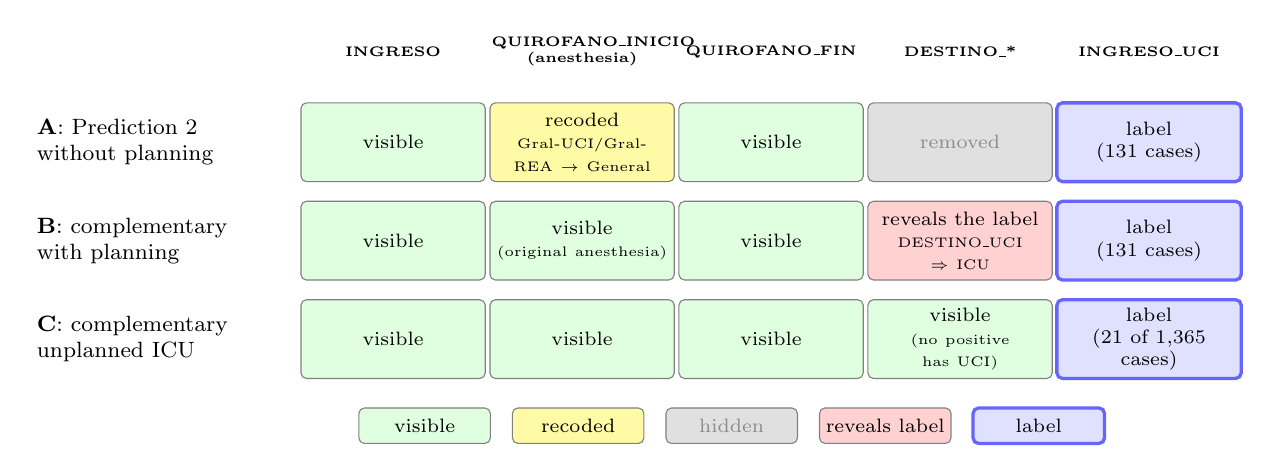
\begin{tikzpicture}[
  ev/.style={draw=black!50, rounded corners=2pt, text width=2.2cm, minimum height=1.0cm, align=center, font=\scriptsize, inner sep=2pt},
  vis/.style={ev, fill=green!12}, rec/.style={ev, fill=yellow!35}, hid/.style={ev, fill=black!12, text=black!45}, rev/.style={ev, fill=red!18}, lab/.style={ev, fill=blue!12, draw=blue!60, very thick},
  rowlab/.style={font=\footnotesize, align=left, text width=3.0cm},
  hdr/.style={font=\tiny\bfseries, align=center, text width=2.3cm}]
% headers
\foreach \x/\h in {0/{\code{INGRESO}},2.4/{\code{QUIROFANO\_INICIO}\\(anesthesia)},4.8/{\code{QUIROFANO\_FIN}},7.2/{\code{DESTINO\_*}},9.6/{\code{INGRESO\_UCI}}} \node[hdr] at (\x,0) {\h};
% row A
\node[rowlab, anchor=east] at (-1.4,-1.15) {\textbf{A}: Prediction~2\\without planning};
\node[vis] at (0,-1.15) {visible};
\node[rec] at (2.4,-1.15) {recoded\\{\tiny\code{Gral-UCI}/\code{Gral-REA} $\to$ General}};
\node[vis] at (4.8,-1.15) {visible};
\node[hid] at (7.2,-1.15) {removed};
\node[lab] at (9.6,-1.15) {label\\(131 cases)};
% row B
\node[rowlab, anchor=east] at (-1.4,-2.4) {\textbf{B}: complementary\\with planning};
\node[vis] at (0,-2.4) {visible};
\node[vis] at (2.4,-2.4) {visible\\{\tiny(original anesthesia)}};
\node[vis] at (4.8,-2.4) {visible};
\node[rev] at (7.2,-2.4) {reveals the label\\{\tiny\code{DESTINO\_UCI} $\Rightarrow$ ICU}};
\node[lab] at (9.6,-2.4) {label\\(131 cases)};
% row C
\node[rowlab, anchor=east] at (-1.4,-3.65) {\textbf{C}: complementary\\unplanned ICU};
\node[vis] at (0,-3.65) {visible};
\node[vis] at (2.4,-3.65) {visible};
\node[vis] at (4.8,-3.65) {visible};
\node[vis] at (7.2,-3.65) {visible\\{\tiny(no positive has \code{UCI})}};
\node[lab] at (9.6,-3.65) {label\\(21 of 1,365 cases)};
% legend
\foreach \x/\s/\t in {0.4/vis/visible, 2.35/rec/recoded, 4.3/hid/hidden, 6.25/rev/{reveals label}, 8.2/lab/label}
  \node[\s, text width=1.6cm, minimum height=0.45cm, inner sep=1pt] at (\x,-4.75) {\t};
\end{tikzpicture}
\caption{The three ways of asking whether the patient will be admitted to the ICU: what the model sees in the prefix in variants A, B and C.}
\label{fig:niveles_abc}
\end{figure}

The design also makes explicit how the Entropy-Driven Next Activity Prediction Approach \cite{zare2025} is transferred to this work (Table~\ref{tab:zare_traslado}). Three elements are kept unchanged: the five algorithms, the process entropy as the measure that characterizes the event log, and next-activity prediction as the reference prediction, which allows a direct comparison with the results table of the paper. One element is added: the two outcome-based predictions that answer the clinical question of the project, which the paper does not address.

\begin{table}[htbp]
\centering
\caption{How the Entropy-Driven Next Activity Prediction Approach of Zare et al.\ is transferred to this work.}
\label{tab:zare_traslado}
\small
\begin{tabular}{L{3.4cm}L{10.2cm}}
\toprule
Element & In this work \\
\midrule
Same algorithm families & DT, RF, XGBoost, LSTM and Transformer, with basic configuration and without hyperparameter search (the paper uses CNN-LSTM and CNN-BiLSTM networks and its own DAW-Transformer). \\
Same measure of the event log & Process entropy: 3.39 bits (3.54 with start and end markers), in the medium band of the paper (Section~\ref{sec:entropia}). \\
Same prediction & Prediction~1 (F), next-activity prediction, comparable with the results table of the paper. \\
Added & Predictions~2 (A) and 3 (E), ICU admission without planning information and prolonged length of stay: the outcome-based predictions that answer the clinical question (FTR), which the paper does not cover. \\
\bottomrule
\end{tabular}
\end{table}

\subsection{Prefixes and Cutting Rules}
\label{sec:prefijos}

The models do not predict from complete traces but from prefixes, because the purpose of PPM is to predict while the case is still running. A prefix is the trace of an episode up to its $k$-th event, with $k = 1 \ldots 6$; the median of the event log is five events, and therefore six prefixes cover practically the whole history of each case. Each prefix is a prediction instance: with $k=1$ the prediction is made at the time of admission, with $k=3$ just after the operating theater. To avoid leakage, no prefix ends in \code{ALTA}, \code{EXITUS} or \code{TRASLADO\_OTRO\_HOSPITAL}, and each prediction cuts the trace \emph{before the event that defines its label}. The cutting rule is therefore specific to each prediction, because the event that reveals the label is different in each case:

\begin{itemize}[leftmargin=*]
  \item \textbf{Prediction~1 (F)}: $k = 1 \ldots \min(n-1, 6)$ and the class is activity $k+1$.
  \item \textbf{Prediction~2 (A)}: before the first \code{INGRESO\_UCI}. The \code{DESTINO\_*} events are removed and the anesthesia \code{Gral-UCI} or \code{Gral-REA} is recoded as General, because both are the decision to reserve a bed.
  \item \textbf{Prediction~3 (E)}: the prefix does not end in an end event and is discarded when the time elapsed since admission already exceeds 8.74 days, because at that point the label is known. No intermediate event is leakage for the length of stay, and therefore all of them are kept, destination included.
  \item \textbf{Complementary analysis D}: before the first postoperative \code{INGRESO\_UCI} or specialist consultation (\code{INTERCONSULTA\_ESPECIALISTA}), \code{EXITUS} or \code{TRASLADO\_OTRO\_HOSPITAL}; preoperative consultations are kept.
\end{itemize}

After applying these rules, Prediction~1 yields 6,013 prefixes with 13 possible classes; Prediction~2, 4,457 prefixes, of which 334 belong to cases that end in the ICU (the positives); and Prediction~3, 5,987 prefixes, of which 721 belong to cases with a prolonged stay. The number of prefixes is larger than the number of cases because each case contributes up to six prefixes, one per prediction point.

\subsection{Encodings}

A prefix is a sequence of events with heterogeneous attributes, and each family of models needs it in a different form: the tree-based models need a fixed-length numeric vector, whereas the neural networks can consume the sequence itself. For this reason the two usual encodings of PPM, introduced in Section~\ref{sec:ppm}, were used. The \textbf{aggregate} encoding, for the tree-based models, produces a vector of 59 to 61 variables. It contains, for each of the 14 activities, its count in the prefix and whether it is the last one; the time elapsed since admission and since the previous event; the case attributes known at admission (age, sex, palliative care, hour and day of the week of admission, the eight most frequent services and the eight most frequent ICD chapters as indicators); and the surgery attributes (category, approach, anesthesia and duration) only when the operating theater is already in the prefix. The \textbf{sequence} encoding, for LSTM and Transformer, keeps the sequence of activities as embeddings with two temporal features per event (logarithm of the time since admission and since the previous event), padded to six positions, and concatenates the same static case vector before the output layer. The next subsection describes this second encoding in detail, because it determines what the sequence models can and cannot learn.

\subsection{Event Encoding for the Sequence Models}
\label{sec:encoding}

The sequence models do not receive the 59--61 aggregate variables but a tensor of fixed shape, six positions by $d$ values, built as Figure~\ref{fig:encoding} shows. Three transformations are involved: homogenizing the length of the prefixes, merging the heterogeneous attributes of each event into a single vector, and keeping the static attributes of the case apart from the sequence.

\paragraph{Length.} Prefixes have between one and six events. All of them are padded to six positions with the reserved activity code 0 and zero temporal features, so that every prefix is a tensor of the same size. In the Transformer, the padding positions are excluded from the attention through a key padding mask and from the final pooling, and therefore a prefix of two events and a prefix of six events yield comparable representations; in the LSTM, the padding is simply read as a neutral token.

\paragraph{Event representation.} In the Transformer each event $i$ of the prefix is represented by a vector $h_i \in \mathbb{R}^{32}$ that is the sum of three learned vectors, as Equation~\ref{eq:encoding} shows:
\begin{equation}
  h_i = \mathrm{Emb}(a_i) + W x_i + p_i .
  \label{eq:encoding}
\end{equation}
The first term is the \textbf{activity embedding}. The activity is first mapped to an integer according to the fixed list of the 14 activities of the event log, from 1 for \code{INGRESO} to 14 for \code{ALTA}. That integer indexes a $15 \times 32$ table whose rows are initialized at random and adjusted by backpropagation. It is not a one-hot encoding: the network learns which 32 numbers represent each activity. The second term is the \textbf{temporal projection}. Two real features are computed per event, the logarithm of one plus the hours elapsed since admission and the logarithm of one plus the hours elapsed since the previous event (zero for the first event); the logarithm compresses the long tail of hospital durations, from minutes in the operating theater to days of stay. A linear layer with a $2 \times 32$ weight matrix and a bias brings these two values into the same 32-dimensional space as the embedding, so that both can be added. The third term is a \textbf{learned positional encoding}, a $6 \times 32$ parameter with one vector per position of the prefix, initialized with a normal distribution of standard deviation 0.02 and trained with the rest. It supplies the notion of order that the attention mechanism lacks on its own, so that \code{QUIROFANO\_FIN} in the second position is not the same as in the fourth. In the LSTM the same inputs are used, but the activity embedding has 16 dimensions and is concatenated with the two temporal features, giving 18 values per event, since a recurrent network does not require all its inputs to share one dimension and obtains the order from the recurrence itself.

\paragraph{Static attributes.} The attributes of the patient and of the surgery (age, sex, palliative care, hour and day of admission, service, ICD chapter, and category, approach, anesthesia and duration of the surgery when the operating theater is already in the prefix) are not events, and therefore they do not enter the sequence. They form a separate vector that is concatenated with the output of the sequence (the mean of the Transformer vectors over the real positions, or the final hidden state of the LSTM) immediately before the output head, a dense layer of 64 units with rectified linear unit (ReLU) activation and dropout of 0.2 followed by the output layer. This is the same information that the tree-based models receive in the aggregate encoding, and therefore the models are compared with the same information.

\paragraph{Size.} The representation of the events in the Transformer uses 768 parameters (the $15 \times 32$ table, the $2 \times 32$ matrix with its 32 biases and the $6 \times 32$ positional parameter). The rest of the model consists of the two encoder layers, with four attention heads of eight dimensions each and a feed-forward network (FFN) of 64 units, and the head. The dimension $d = 32$ is deliberately small compared with the 256 of the DAW-Transformer of Zare et al.\ \cite{zare2025}: with 14 activities, prefixes of at most six events and between four and six thousand prefixes, a larger model would add parameters without data to fit them.

\begin{figure}[htbp]
\centering
\begin{tikzpicture}[
  box/.style={draw=black!60, rounded corners=2pt, align=center, font=\scriptsize, inner sep=3pt},
  slot/.style={box, text width=1.75cm, minimum height=0.75cm, fill=black!4, inner sep=1pt},
  pad/.style={slot, fill=black!10, text=black!45, dashed},
  comp/.style={box, text width=3.3cm, minimum height=0.85cm},
  emb/.style={comp, fill=blue!10}, tim/.style={comp, fill=orange!15}, posn/.style={comp, fill=green!12}, sum/.style={circle, draw, inner sep=1pt, font=\small},
  blk/.style={box, text width=7.6cm, minimum height=0.75cm, fill=black!5},
  arr/.style={-{Latex[length=1.6mm]}, black!60}]
% prefix slots
\node[font=\footnotesize, anchor=west] at (-0.95,1.05) {Prefix padded to six positions ($k = 3$ in the example):};
\foreach \i/\t/\s in {0/{{\tiny\code{INGRESO}}\\$a_1{=}1,\ x_1{=}0$}/slot, 1/{{\tiny\code{QUIROFANO\_INICIO}}\\$a_2 = 4,\ x_2$}/slot, 2/{{\tiny\code{QUIROFANO\_FIN}}\\$a_3 = 5,\ x_3$}/slot, 3/{padding\\$a_4 = 0$}/pad, 4/{padding\\$a_5 = 0$}/pad, 5/{padding\\$a_6 = 0$}/pad}
  \node[\s] (p\i) at (\i*1.95,0) {\t};
% three components for event i
\node[emb] (e) at (1.3,-1.9) {$\mathrm{Emb}(a_i)$: embedding table\\$15 \times 32$, row 0 = padding};
\node[tim] (w) at (4.9,-1.9) {$W x_i$: linear layer $2 \to 32$\\$x_i = (\log(1+\Delta t_{\mathrm{adm}}),\ \log(1+\Delta t_{\mathrm{prev}}))$};
\node[posn] (q) at (8.5,-1.9) {$p_i$: learned positional vector\\$6 \times 32$ parameter};
\node[sum] (s) at (4.9,-3.05) {$+$};
\draw[arr] (e.south) -- (s); \draw[arr] (w.south) -- (s); \draw[arr] (q.south) -- (s);
\draw[arr, dashed] (p1.south) -- ++(0,-0.3) -| (e.north);
\draw[arr, dashed] (p1.south) -- ++(0,-0.3) -| (w.north);
\node[font=\scriptsize, anchor=west] at (5.25,-3.05) {$h_i \in \mathbb{R}^{32}$, one vector per position};
% encoder and head
\node[blk] (enc) at (4.9,-4.1) {Transformer encoder: 2 layers, 4 heads, FFN 64, dropout 0.1;\\padding positions excluded from the attention (\code{src\_key\_padding\_mask})};
\node[blk] (pool) at (4.9,-5.3) {Mean pooling over the real positions only $\to$ one vector of 32 for the prefix};
\node[box, fill=yellow!20, text width=2.9cm, minimum height=0.75cm] (st) at (10.75,-5.3) {Static case vector\\{\tiny age, sex, service, ICD chapter, surgery attributes}};
\node[blk] (head) at (4.9,-6.45) {Concatenation $[\,32 + n_{\mathrm{static}}\,] \to$ Dense 64 $\to$ ReLU $\to$ Dropout 0.2 $\to$ output};
\draw[arr] (s) -- (enc); \draw[arr] (enc) -- (pool); \draw[arr] (pool) -- (head); \draw[arr] (st.south) |- ([yshift=0.12cm]head.east);
\node[font=\scriptsize, align=left, anchor=north west, text width=12.6cm] at (-0.95,-7.1) {LSTM: same inputs, but the 16-dimensional embedding and $x_i$ are concatenated (18 values per event) and fed to an LSTM with 64 units; the static vector is concatenated to the final hidden state in the same way.};
\end{tikzpicture}
\caption{Encoding of a prefix for the sequence models. Each event is represented by the sum of three learned vectors of 32 dimensions; the static attributes of the case enter only after the pooling.}
\label{fig:encoding}
\end{figure}

\subsection{Split, Threshold and Seeds}

The evaluation protocol has to reproduce the situation in which the models would be used: trained on past cases and applied to new ones. The split is therefore \textbf{temporal by admission date, at case level}: the oldest 64\% of the cases train, the next 16\% serve as validation (early stopping and threshold selection) and the most recent 20\% (295 cases) form the test set. All the prefixes of a case fall in the same partition, so that the model never sees in training a prefix of a case that is evaluated in test. The decision threshold is chosen on validation by maximizing F1-score and applied on test. Each experiment is repeated with three seeds (0, 1 and 2) and the mean and standard deviation are reported. The prevalences quoted with the results are those of the test set, which differ slightly from the population prevalences of Table~\ref{tab:etiquetas}.

\subsection{Models}

Table~\ref{tab:modelos} shows the configuration of the five algorithms. It is deliberately basic and common to all the predictions: the comparison is between model families, not between tuning efforts, and this is also the setting of the Entropy-Driven Next Activity Prediction Approach, which uses the algorithms without hyperparameter search. The tree-based models use the implementations of scikit-learn and of the XGBoost library; the two neural networks were implemented in PyTorch and trained with the Adam optimizer, early stopping on the validation set and the same number of maximum epochs. Class imbalance is handled with class weights in the models, never with subsampling: each model gives more weight to the errors on the minority class (\code{class\_weight} and \code{balanced\_subsample} in the tree-based models, \code{scale\_pos\_weight} in XGBoost and \code{pos\_weight} in the loss of the networks), so that the training data are not altered.

\begin{table}[htbp]
\centering
\caption{Basic configuration of the five algorithms.}
\label{tab:modelos}
\small
\begin{tabular}{L{2.2cm}L{5.5cm}L{1.7cm}L{3.4cm}}
\toprule
Model & Configuration & Input & Imbalance \\
\midrule
DT & Maximum depth 6, minimum 5 samples per leaf & Aggregate & balanced \code{class\_weight} \\
RF & 300 trees, minimum 3 samples per leaf & Aggregate & \code{balanced\_subsample} \\
XGBoost & 400 trees, depth 4, learning rate 0.05, subsampling 0.9 / 0.8, early stopping at 30 rounds & Aggregate & \code{scale\_pos\_weight} \\
LSTM & Embedding 16 $\rightarrow$ LSTM 64 $\rightarrow$ [h ; static] $\rightarrow$ 64 $\rightarrow$ output; Adam $10^{-3}$, up to 80 epochs, early stopping 12 & Sequence & \code{pos\_weight} in the loss \\
Transformer & $d = 32$, 4 heads, 2 layers, FFN 64, dropout 0.1, learned positional encoding, mean pooling; same training & Sequence & \code{pos\_weight} in the loss \\
\bottomrule
\end{tabular}
\end{table}

\subsection{Metrics}

For Prediction~1 (next activity), accuracy, macro F1-score and weighted F1-score are used. The baseline predicts the most frequent transition from the last activity, as in the Entropy-Driven Next Activity Prediction Approach \cite{zare2025}. For the outcome-based predictions (Predictions~2 and 3), the reported metrics are AUC-ROC, AUC-PR, F1-score, recall and precision at the chosen threshold, the Brier score and AUC-ROC per prefix length (when there are at least three positives and three negatives in test). The variable importance of RF and XGBoost is also reported, shown as a figure for Predictions~2 and 3. AUC-ROC and the per-prefix evaluation follow the benchmark of Teinemaa et al.\ \cite{teinemaa2019}; AUC-PR is added because with 8--12\% positives the ROC is dominated by the negatives \cite{saito2015}; and the Brier score because in a clinical context a calibrated probability matters.

\section{Prediction 1: Next Activity}

Prediction~1, the next activity of the case and the reference prediction of the Entropy-Driven Next Activity Prediction Approach \cite{zare2025}, uses 6,013 prefixes and 13 classes (all the activities except \code{INGRESO}). The distribution is very uneven: \code{ALTA} (1,403), \code{QUIROFANO\_INICIO} (1,373), \code{QUIROFANO\_FIN} (1,366) and \code{DESTINO\_PLANTA} (1,184) concentrate most of the instances, versus five classes with fewer than 20 instances among the prefixes: the transfer to the ward, the consultation to the ICU, the destination \code{DESTINO\_OTROS}, death and the transfer to another hospital. Table~\ref{tab:tarea1} presents the results, Figure~\ref{fig:confusion} the confusion matrix of the best model and Table~\ref{tab:tarea1_k} the accuracy by prefix length.

\begin{table}[htbp]
\centering
\caption{Prediction 1: test results against the most-frequent-transition baseline.}
\label{tab:tarea1}
\begin{tabular}{lcccc}
\toprule
Model & Accuracy & Macro F1 & Weighted F1 & Time (s) \\
\midrule
Baseline & 0.867 & 0.399 & -- & -- \\
DT (balanced) & 0.746 $\pm$ 0.001 & 0.352 $\pm$ 0.000 & 0.807 & 0.0 \\
RF & 0.883 $\pm$ 0.002 & 0.527 $\pm$ 0.001 & 0.893 & 2.1 \\
XGBoost & 0.906 $\pm$ 0.002 & 0.518 $\pm$ 0.003 & 0.903 & 2.3 \\
LSTM & \textbf{0.913} $\pm$ 0.000 & \textbf{0.529} $\pm$ 0.004 & \textbf{0.909} & 12.7 \\
Transformer & 0.912 $\pm$ 0.005 & 0.526 $\pm$ 0.009 & 0.907 & 38.0 \\
\bottomrule
\end{tabular}
\end{table}

\begin{figure}[htbp]
\centering
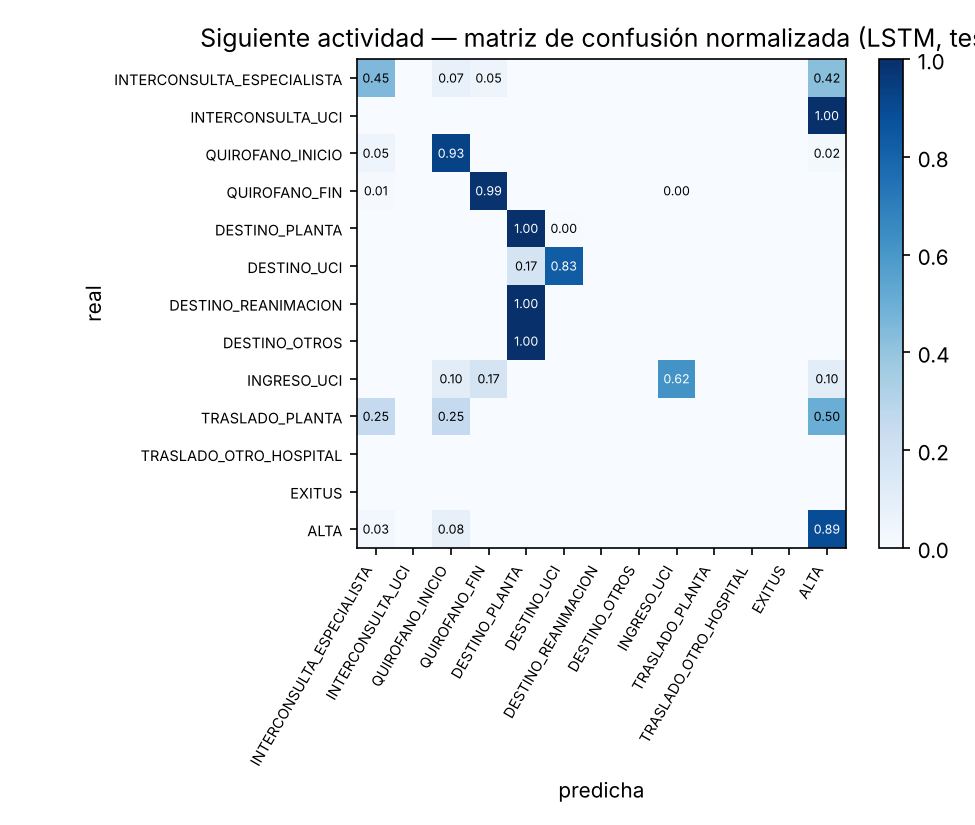
\includegraphics[width=0.75\textwidth]{nextact_confusion}
\caption{Prediction 1: row-normalized confusion matrix of the LSTM on test.}
\label{fig:confusion}
\end{figure}

The best models reach \textbf{0.91 accuracy, 4.6 points above the baseline}. The improvement comes from the fact that the destination decision, although newly added to the event log, is largely predictable: 87\% of the destinations are the ward and the \code{Gral-UCI} anesthesia anticipates \code{DESTINO\_UCI} in 88 of 122 interventions. By contrast, the \code{Gral-REA} anesthesia mostly ends in the ward (128 of 171), and therefore the post-anesthesia care unit is the exit of the operating theater that is worst predicted. The rare classes are not learned, hence the macro F1-score of 0.52--0.53; the DT with balanced weights sacrifices accuracy in favor of the rare classes. Compared with the results table of Zare et al.\ \cite{zare2025} (94\% on Helpdesk, 97\% on BPIC 2017, 60--70\% on Sepsis), the event log behaves as one of intermediate difficulty, consistent with its 3.39 bits of entropy.

\begin{table}[htbp]
\centering
\caption{Prediction 1: accuracy by prefix length on test, mean of three seeds.}
\label{tab:tarea1_k}
\small
\begin{tabular}{lrcccccc}
\toprule
$k$ & $n$ & Baseline & DT & RF & XGBoost & LSTM & Transformer \\
\midrule
1 (admission) & 295 & 0.868 & 0.834 & 0.859 & \textbf{0.875} & 0.856 & 0.858 \\
2 (in theater) & 269 & 0.922 & 0.836 & 0.908 & \textbf{0.943} & 0.939 & 0.938 \\
3 (after theater) & 265 & 0.883 & 0.616 & 0.887 & 0.923 & \textbf{0.971} & 0.970 \\
4 & 263 & 0.920 & 0.795 & \textbf{0.943} & 0.942 & 0.937 & 0.938 \\
5 & 53 & 0.415 & 0.415 & 0.679 & 0.742 & \textbf{0.805} & 0.786 \\
6 & 17 & 0.353 & 0.118 & 0.549 & \textbf{0.588} & 0.569 & 0.549 \\
\midrule
All & 1,162 & 0.867 & 0.746 & 0.883 & 0.906 & \textbf{0.913} & 0.912 \\
\bottomrule
\end{tabular}
\end{table}

Table~\ref{tab:tarea1_k} shows where the advantage of the models over the baseline comes from. At admission ($k=1$) the next event is almost always the operating theater and no model beats the trivial prediction by more than one point. The difference concentrates at the exit of the operating theater ($k=3$), where the next activity is the planned destination: the sequence models reach 0.97 against 0.88 for the baseline, because the anesthesia recorded at the start of the surgery anticipates the destination and the sequence models exploit it better than the tree-based models, which stay at 0.89--0.92. From $k=5$ onward, with 53 and 17 prefixes, the cases are the complicated episodes with consultations, ICU admissions and transfers, and the accuracy of every model except DT drops to 0.55--0.80; there the baseline collapses to 0.35--0.42, which shows that the models do learn something about the atypical trajectories even though they have few examples of them.

\section{Prediction 2: ICU Admission Without Planning Information}
\label{sec:pred2}

Table~\ref{tab:tarea2} presents the test results (860 prefixes, 70 positives, prevalence 8.1\%) and Figure~\ref{fig:tarea2_curvas} the ROC and precision--recall curves.

\begin{table}[htbp]
\centering
\caption{Prediction 2: test results, mean $\pm$ standard deviation over three seeds.}
\label{tab:tarea2}
\small
\begin{tabular}{lccccccc}
\toprule
Model & AUC-ROC & AUC-PR & F1 & Recall & Prec. & Brier & Time (s) \\
\midrule
DT & 0.754 $\pm$ 0.002 & 0.205 $\pm$ 0.004 & 0.291 & 0.34 & 0.25 & 0.165 & 0.0 \\
RF & 0.876 $\pm$ 0.002 & 0.399 $\pm$ 0.007 & 0.395 & 0.45 & 0.39 & \textbf{0.081} & 2.0 \\
XGBoost & 0.846 $\pm$ 0.005 & 0.280 $\pm$ 0.001 & 0.362 & 0.41 & 0.34 & 0.111 & 0.3 \\
LSTM & \textbf{0.886} $\pm$ 0.003 & \textbf{0.413} $\pm$ 0.014 & 0.448 & 0.51 & 0.40 & 0.161 & 22.2 \\
Transformer & \textbf{0.886} $\pm$ 0.004 & 0.411 $\pm$ 0.008 & \textbf{0.455} & 0.47 & 0.44 & 0.139 & 38.6 \\
\bottomrule
\end{tabular}
\end{table}

\begin{figure}[htbp]
\centering
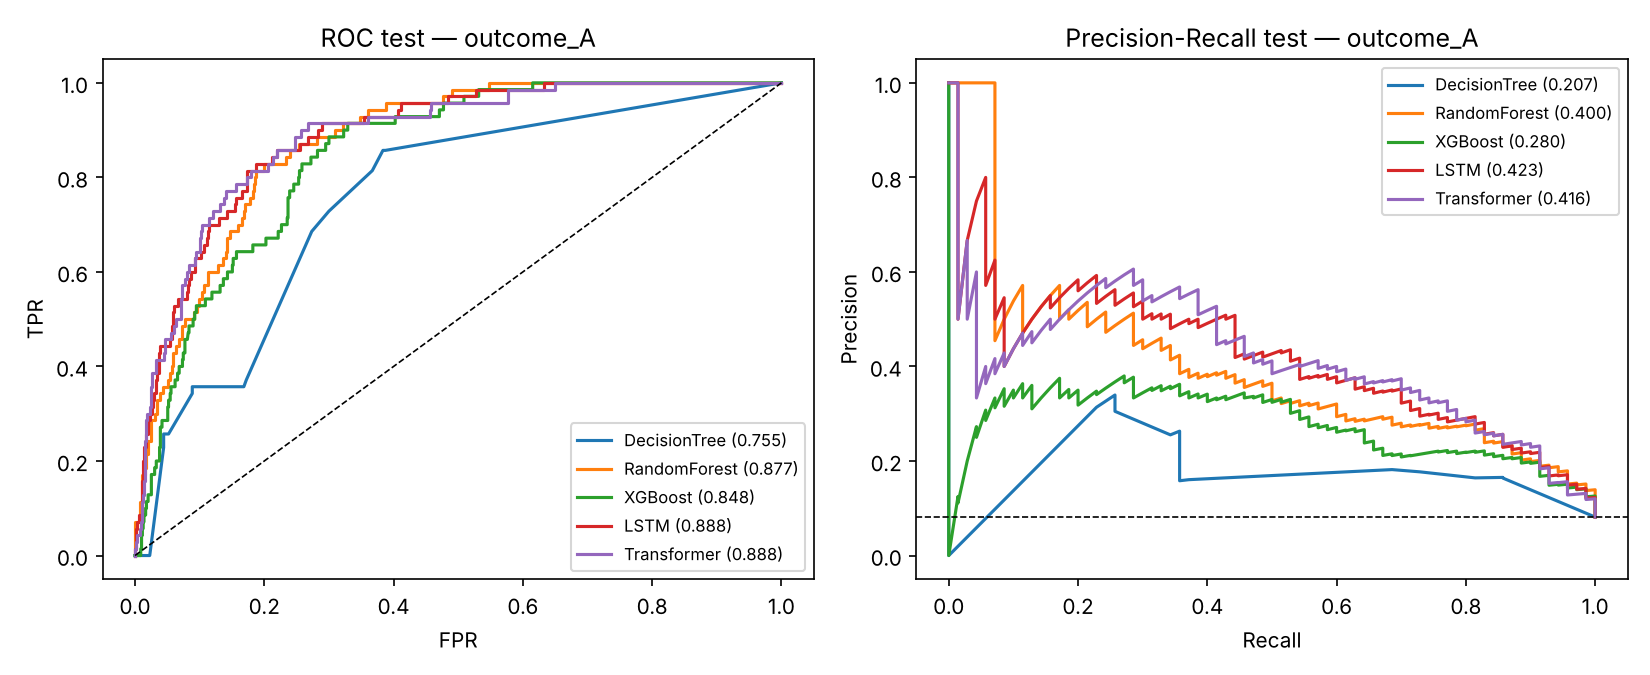
\includegraphics[width=\textwidth]{outcome_A_curvas}
\caption{Prediction 2: ROC and precision--recall curves on test.}
\label{fig:tarea2_curvas}
\end{figure}

Without the planning information, ICU admission is \textbf{predictable in a useful but not excellent way}: AUC-ROC of 0.85 to 0.89 and AUC-PR of 0.40, five times the prevalence of 8.1\%, which is the value a random classifier would obtain. LSTM and Transformer are one point above RF in AUC-ROC and on a par in AUC-PR, whereas RF is clearly the best calibrated: its Brier score of 0.081 is half that of the sequence models (0.161 for LSTM and 0.139 for Transformer), with XGBoost at 0.111 and DT at 0.165. DT and XGBoost with basic configuration are clearly behind in ranking. For reference, the same label with the planned destination in the prefix reaches an AUC-ROC of 0.969 overall and of 0.999 once the destination is in the prefix (complementary B, Section~\ref{sec:compl_b}); the gap between those values and 0.886 is exactly the planning information that variant A hides.

Table~\ref{tab:tarea2_k} and Figure~\ref{fig:tarea2_k} show how the prediction evolves with the prefix length, and Figure~\ref{fig:tarea2_imp} the variable importance. Each prefix length corresponds to a clinically meaningful moment: $k=1$ is the time of admission (295 test cases, 26 of them positive), $k=2$ is the entry into the operating theater, when the anesthesia is known (267 cases, 24 positive), and $k=3$ is the exit from the operating theater (258 cases, 19 positive). At admission, with only the patient and the service, 0.83--0.84 is already reached; in the operating theater the best models rise to 0.87--0.91; and after the operating theater to 0.92, because the anesthesia, the duration and the approach add real information about the risk. The test population shrinks with $k$ because the cases that are admitted to the ICU early, or that are discharged, stop producing prefixes.

\begin{table}[htbp]
\centering
\caption{Prediction 2: AUC-ROC per prefix length on test.}
\label{tab:tarea2_k}
\small
\begin{tabular}{lcccccc}
\toprule
$k$ & $n$ (positives) & DT & RF & XGBoost & LSTM & Transformer \\
\midrule
1 (admission) & 295 (26) & 0.723 & \textbf{0.843} & 0.799 & 0.832 & 0.825 \\
2 (in theater) & 267 (24) & 0.773 & 0.870 & 0.844 & 0.897 & \textbf{0.905} \\
3 (after theater) & 258 (19) & 0.773 & 0.921 & 0.894 & \textbf{0.924} & \textbf{0.924} \\
\bottomrule
\end{tabular}
\end{table}

\begin{figure}[htbp]
\centering
\begin{subfigure}[t]{0.56\textwidth}
\centering
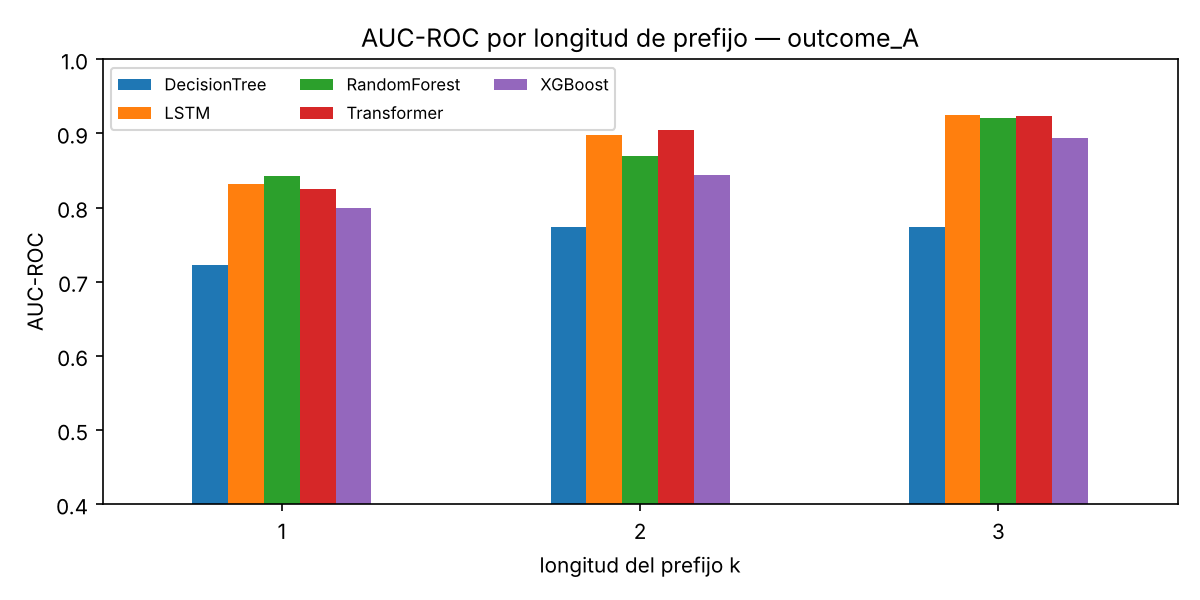
\includegraphics[width=\textwidth]{outcome_A_auc_por_prefijo}
\caption{AUC-ROC per prefix length.}
\label{fig:tarea2_k}
\end{subfigure}
\hfill
\begin{subfigure}[t]{0.42\textwidth}
\centering
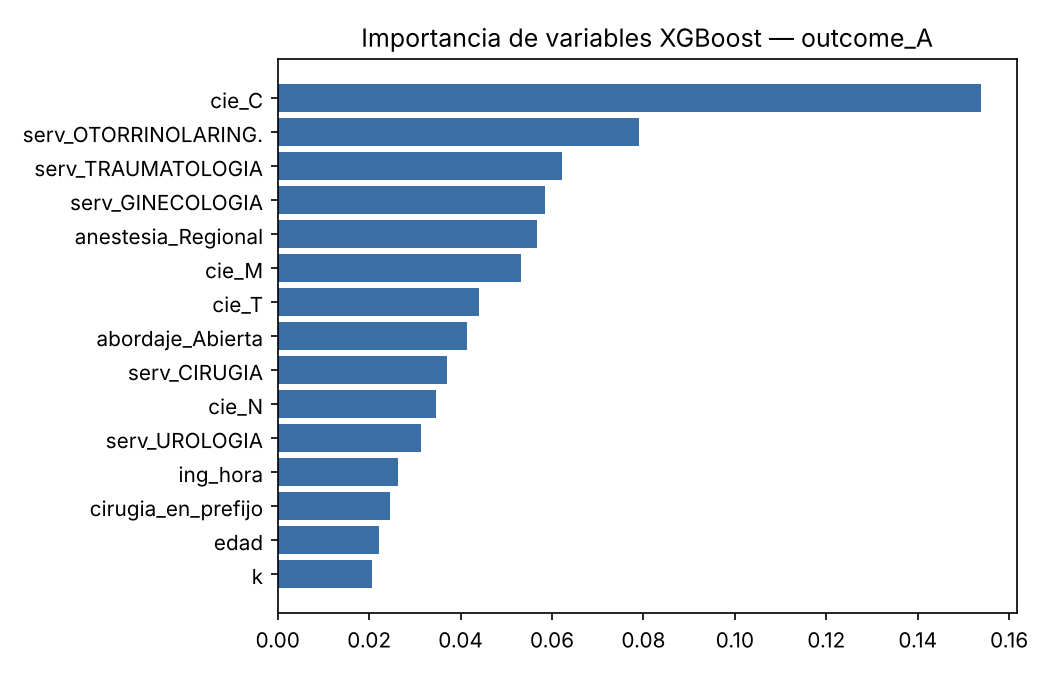
\includegraphics[width=\textwidth]{outcome_A_importancia_xgb}
\caption{Variable importance (XGBoost).}
\label{fig:tarea2_imp}
\end{subfigure}
\caption{Prediction 2: evolution with the prefix and variable importance.}
\label{fig:tarea2_evol}
\end{figure}

The most important variables (Figure~\ref{fig:tarea2_imp}) are, for RF, ICD chapter C (neoplasms, importance 0.12), age (0.12), the hour of admission (0.10), the elapsed times (0.07), the day of the week, and the orthopedics and otorhinolaryngology services as low-risk indicators. For XGBoost, the most important are chapter C again (0.15), otorhinolaryngology, orthopedics and gynecology, regional anesthesia, chapters M and T, and the open approach. The signal lies in the patient and surgery attributes, not in the order of the events, which explains why the tree-based models come so close to the networks. The results agree with those obtained on version 2 of the event log (0.85--0.88): variant A contains the same information, and therefore the new event log changes nothing when the destination is ignored.

\section{Prediction 3: Prolonged Length of Stay}

Prolonged length of stay is defined as a stay above the 90th percentile of the population, 8.74 days (148 cases). Table~\ref{tab:tarea3} and Figure~\ref{fig:tarea3_curvas} report the test results (1,160 prefixes, 137 positives, prevalence 11.8\%).

\begin{table}[htbp]
\centering
\caption{Prediction 3: test results, mean $\pm$ standard deviation over three seeds.}
\label{tab:tarea3}
\small
\begin{tabular}{lccccccc}
\toprule
Model & AUC-ROC & AUC-PR & F1 & Recall & Prec. & Brier & Time (s) \\
\midrule
DT & 0.829 $\pm$ 0.000 & 0.416 $\pm$ 0.000 & 0.569 & 0.64 & 0.51 & 0.148 & 0.0 \\
RF & 0.896 $\pm$ 0.000 & 0.475 $\pm$ 0.012 & 0.581 & 0.60 & 0.57 & \textbf{0.091} & 1.9 \\
XGBoost & 0.883 $\pm$ 0.004 & 0.478 $\pm$ 0.013 & 0.540 & 0.53 & 0.55 & 0.119 & 0.2 \\
LSTM & \textbf{0.901} $\pm$ 0.002 & \textbf{0.547} $\pm$ 0.010 & \textbf{0.606} & 0.64 & 0.58 & 0.127 & 14.3 \\
Transformer & 0.887 $\pm$ 0.002 & 0.533 $\pm$ 0.006 & 0.547 & 0.53 & 0.57 & 0.148 & 28.9 \\
\bottomrule
\end{tabular}
\end{table}

\begin{figure}[htbp]
\centering
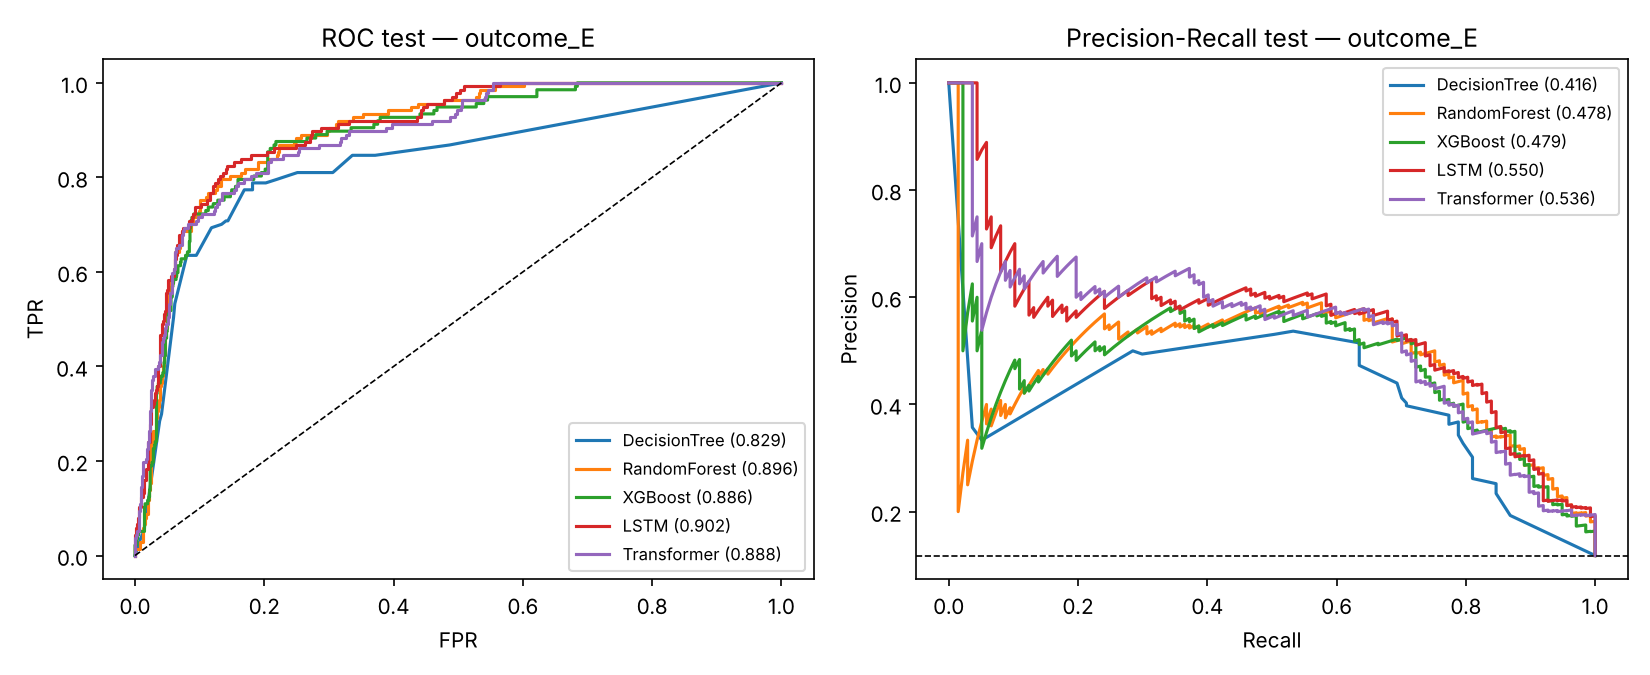
\includegraphics[width=\textwidth]{outcome_E_curvas}
\caption{Prediction 3: ROC and precision--recall curves on test.}
\label{fig:tarea3_curvas}
\end{figure}

Prolonged length of stay is the \textbf{best-predicted target}: AUC-ROC of 0.88 to 0.90 and AUC-PR of 0.47 to 0.55, four to five times the prevalence of 11.8\%, values of the order of those published in the PPM literature for this target. The pattern of Prediction~2 is repeated: LSTM wins in AUC-ROC, AUC-PR and F1-score, RF is half a point behind and is the best calibrated (Brier 0.091, against 0.119 for XGBoost, 0.127 for LSTM and 0.148 for DT and Transformer), and Transformer is slightly behind LSTM. The target depends largely on what is known at admission (the service, with general surgery as the main risk indicator, the type and duration of the surgery and the age) and on the time already elapsed, as the evolution by prefix length in Table~\ref{tab:tarea3_k} shows.

\begin{table}[htbp]
\centering
\caption{Prediction 3: AUC-ROC per prefix length on test.}
\label{tab:tarea3_k}
\begin{tabular}{lcccccc}
\toprule
$k$ & $n$ (positives) & DT & RF & XGBoost & LSTM & Transformer \\
\midrule
1 & 295 (29) & 0.762 & 0.836 & 0.817 & \textbf{0.840} & 0.819 \\
2 & 269 (28) & 0.780 & 0.879 & 0.866 & \textbf{0.899} & 0.882 \\
3 & 265 (28) & 0.840 & \textbf{0.922} & 0.906 & 0.919 & 0.913 \\
4 & 263 (27) & 0.838 & \textbf{0.920} & 0.907 & 0.918 & 0.908 \\
5 & 53 (17) & 0.785 & 0.820 & 0.817 & \textbf{0.842} & 0.840 \\
6 & 15 (8) & 0.688 & 0.589 & 0.696 & 0.732 & \textbf{0.750} \\
\bottomrule
\end{tabular}
\end{table}

By prefix length (Table~\ref{tab:tarea3_k} and Figure~\ref{fig:tarea3_k}), the starting point at admission is 0.82--0.84 and after the operating theater 0.92 is reached. From $k=5$ onward the AUC-ROC drops, but those prefixes are few (53 and 15 in test) and correspond to already complicated episodes, in which a third or a half are positive: distinguishing between patients who have already been admitted for several days is a different and harder problem. Elapsed time is the main variable (importance 0.16 in RF and 0.12 in XGBoost, Figure~\ref{fig:tarea3_imp}); in XGBoost it is followed by the general surgery service, the \code{Gral-UCI} and general anesthesia and the orthopedics service, and in RF by the hour of admission, age, surgery duration, the general surgery service and the \code{Gral-UCI} anesthesia. It is a legitimate variable, since at prediction time it is known how long the patient has been admitted, but it should be made explicit: a prefix that is already on day 7 is almost certainly positive. Run without the planning information, the prediction loses between 1.5 and 2 points of AUC-ROC (LSTM 0.885, RF 0.879): the planned destination informs about the length of stay but does not determine it, and the ranking of the models does not change.

\begin{figure}[htbp]
\centering
\begin{subfigure}[t]{0.56\textwidth}
\centering
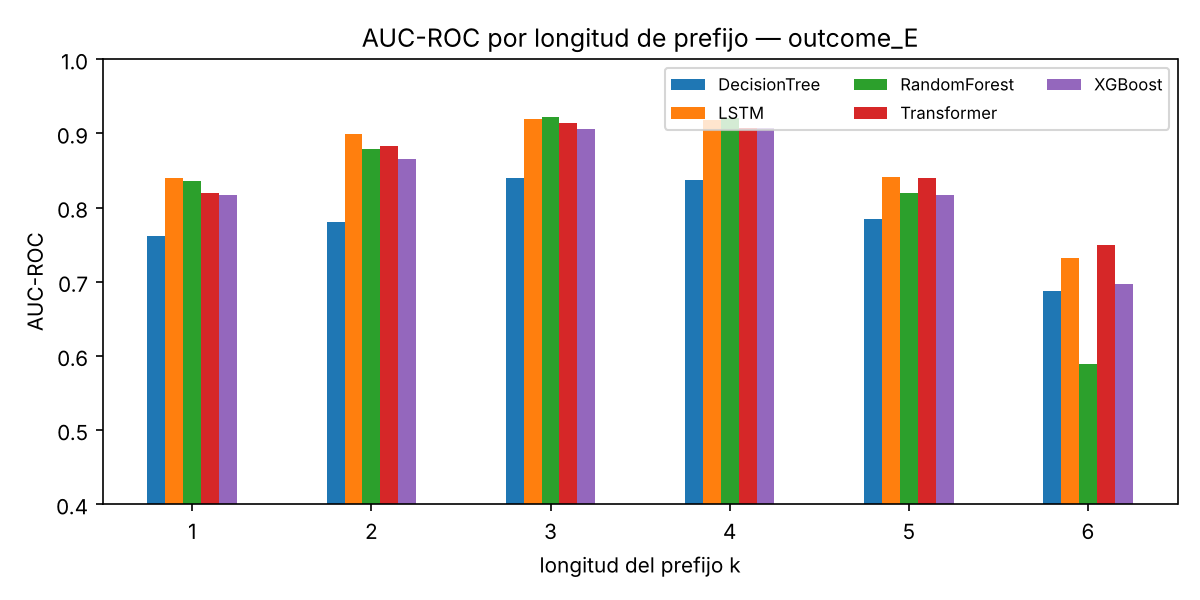
\includegraphics[width=\textwidth]{outcome_E_auc_por_prefijo}
\caption{AUC-ROC per prefix length.}
\label{fig:tarea3_k}
\end{subfigure}
\hfill
\begin{subfigure}[t]{0.42\textwidth}
\centering
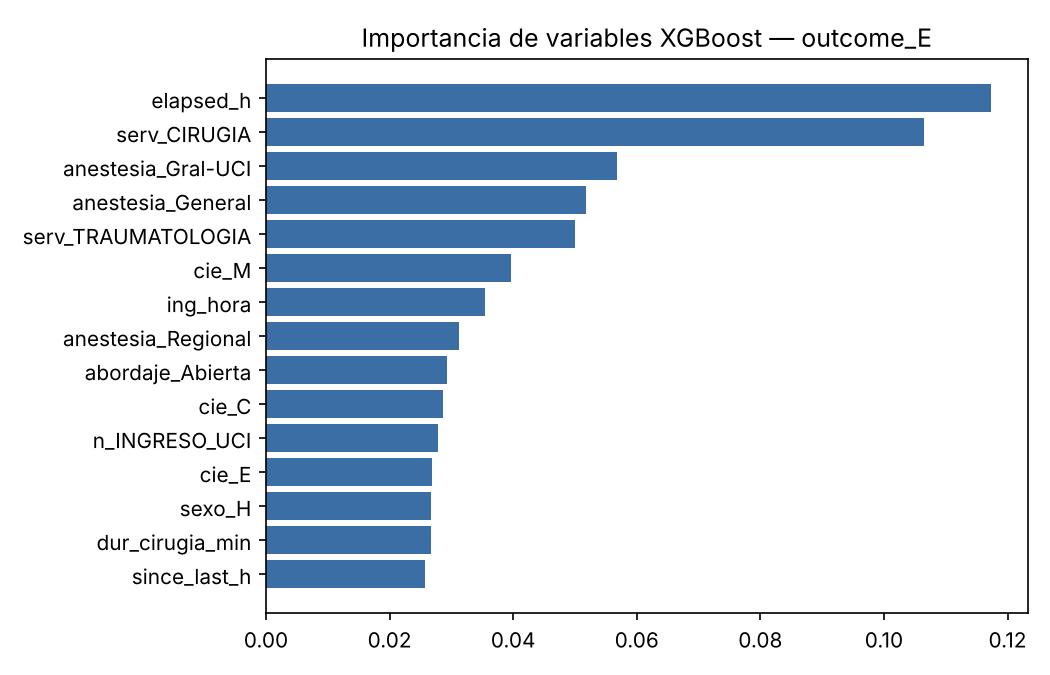
\includegraphics[width=\textwidth]{outcome_E_importancia_xgb}
\caption{Variable importance (XGBoost).}
\label{fig:tarea3_imp}
\end{subfigure}
\caption{Prediction 3: evolution with the prefix and variable importance.}
\label{fig:tarea3_evol}
\end{figure}

\section{Complementary Analyses}

The three predictions above are completed with four complementary analyses, which do not add new predictions but justify the design of Prediction~2 and measure the sensitivity of the results. The first two, B and C, are the other two ways of asking the ICU admission question introduced in Section~\ref{sec:destino_uci}: with the planning information in the prefix (B) and restricted to the unplanned admissions (C). The third, D, evaluates the broad postoperative complication label of Table~\ref{tab:etiquetas}. The fourth measures what happens when the number of coded diagnoses, excluded as leakage in Section~\ref{sec:fugas}, is included.

\subsection{ICU Admission With the Destination in the Prefix (B)}
\label{sec:compl_b}

When Prediction~2 is run with the \code{DESTINO\_*} events and the original anesthesia, AUC-ROC rises to 0.969 (RF) and 0.960 (LSTM), and AUC-PR to 0.80 (Table~\ref{tab:compl_bc}, Figure~\ref{fig:B}). By prefix length, RF goes from 0.844 at admission to 0.978 in the operating theater (with the \code{Gral-UCI} anesthesia) and to \textbf{0.999 once the destination is in the prefix}. With the destination, the prediction is trivial; before the destination, the anesthesia already reveals almost the same. That is why B is not a predictive result but the measure of how much of ICU admission is decided in advance, which is most of it, and why Prediction~2 is variant A.

\begin{table}[htbp]
\centering
\caption{Complementary B and C: AUC-ROC and AUC-PR on test (B) and out of sample with cross-validation (C, prefix at the exit of the operating theater).}
\label{tab:compl_bc}
\begin{tabular}{lcccc}
\toprule
 & \multicolumn{2}{c}{B: with destination} & \multicolumn{2}{c}{C: unplanned ICU} \\
\cmidrule(lr){2-3}\cmidrule(lr){4-5}
Model & AUC-ROC & AUC-PR & AUC-ROC & AUC-PR \\
\midrule
DT & 0.882 & 0.695 & 0.657 $\pm$ 0.053 & 0.035 \\
RF & \textbf{0.969} & \textbf{0.806} & \textbf{0.873} $\pm$ 0.021 & 0.059 \\
XGBoost & 0.936 & 0.744 & 0.635 $\pm$ 0.007 & 0.025 \\
LSTM & 0.960 & 0.800 & 0.679 $\pm$ 0.059 & 0.035 \\
Transformer & 0.956 & 0.785 & 0.715 $\pm$ 0.033 & \textbf{0.070} \\
\bottomrule
\end{tabular}
\end{table}

\begin{figure}[htbp]
\centering
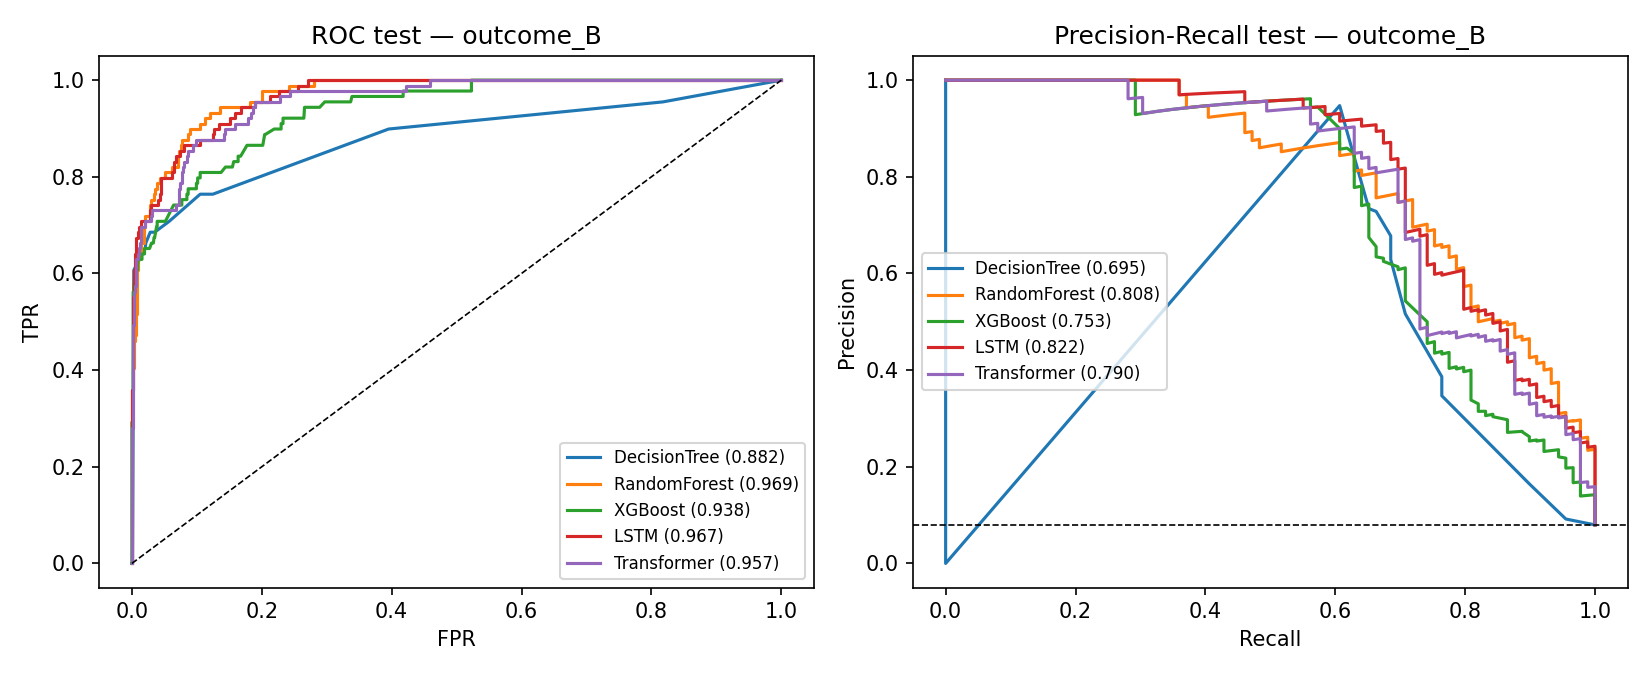
\includegraphics[width=\textwidth]{outcome_B_curvas}
\caption{Complementary B: ROC and precision--recall curves with the destination in the prefix.}
\label{fig:B}
\end{figure}

\subsection{Unplanned ICU Admission (C)}
\label{sec:compl_c}

The target is the 21 episodes that ended up in the ICU without a planned ICU destination, in the population of 1,365 cases without \code{DESTINO\_UCI}; here the planned destination is legitimate information, because no positive has it. With the temporal split the test set would contain only three positives, and therefore the evaluation uses stratified five-fold cross-validation by case with three repetitions, measuring on the prefix ending in \code{DESTINO\_*}, i.e., at the exit of the operating theater (1,220 prefixes, 11 positives, prevalence 0.9\%). RF separates the cases well (AUC-ROC 0.873, Figure~\ref{fig:C}) and assigns the ward patients who ended up in the ICU an average risk four times higher than the rest (0.099 versus 0.023). However, with that prevalence the AUC-PR is 0.06: out of every 15 or 20 alerts, one would be a real case. The deep models and XGBoost do not learn with 21 positives (0.64--0.72). It is the most clinically relevant target, but with 21 cases it allows only an exploratory analysis.

\begin{figure}[htbp]
\centering
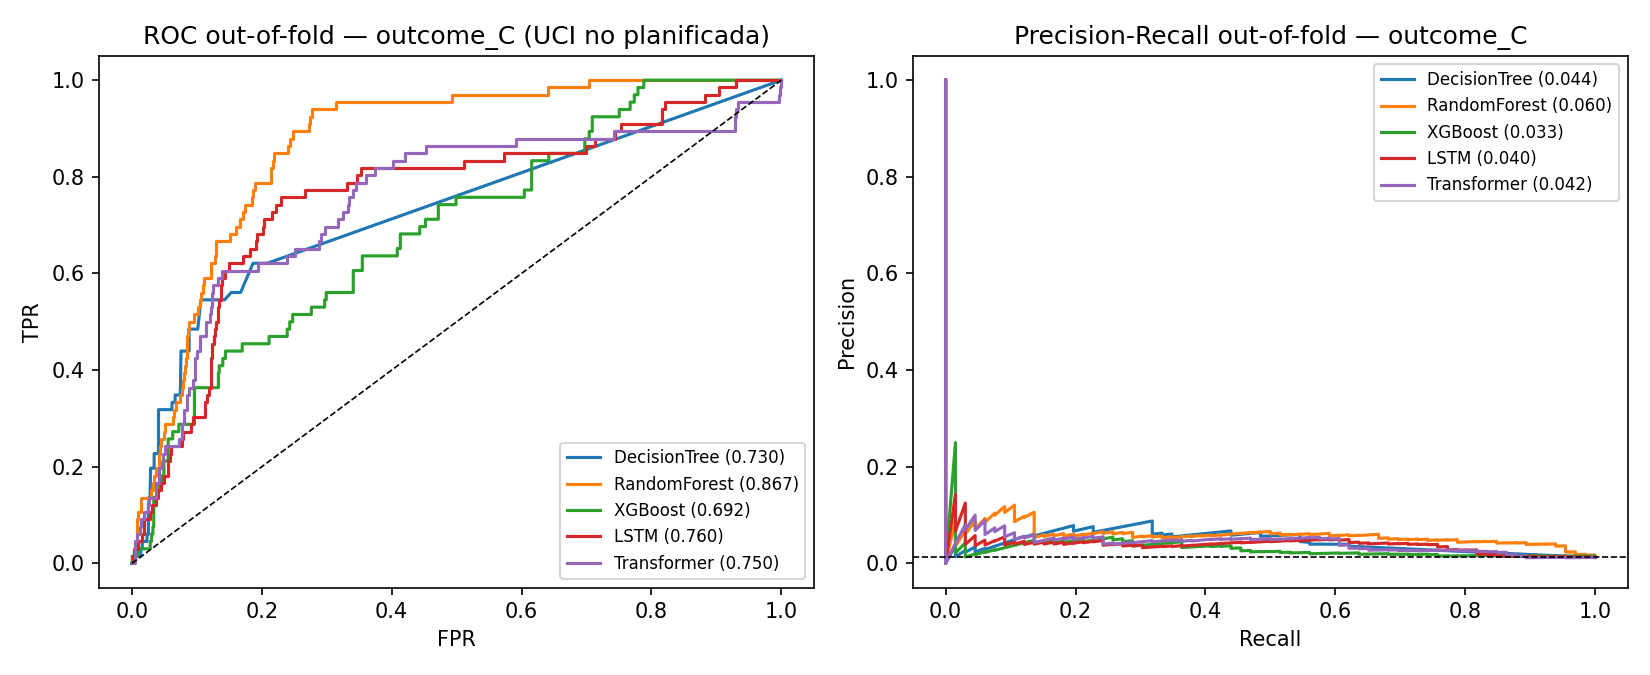
\includegraphics[width=\textwidth]{outcome_C_cv_curvas}
\caption{Complementary C: out-of-sample curves (cross-validation) for unplanned ICU admission.}
\label{fig:C}
\end{figure}

\subsection{The Broad Postoperative Complication (D)}

The postoperative complication label (240 cases: 114 postoperative ICU admissions, 165 postoperative specialist consultations, nine deaths and one transfer) was tested with the same recipe as Prediction~2. It is the hardest target (Table~\ref{tab:D}, Figure~\ref{fig:D}): AUC-ROC of 0.76 to 0.78 and AUC-PR of 0.37 to 0.42, three times the prevalence (13.2\%). It is also the only one in which the tree-based models beat the deep models: RF is the best in all metrics and the sequence models are two points below. The reason lies in the label: two thirds of the positives are postoperative consultations, a soft event that may be routine rather than complication, and 105 are planned ICU admissions (105 of the 110 cases with destination ICU; in the other five the transfer is recorded before the first surgery and does not count as postoperative). With the destination in the prefix RF rises to 0.845 / 0.636, far from the 0.999 of B: the unplanned part of the complication remains hard with or without destination. By prefix length, the signal is already present at the entry into the operating theater ($k=2$, AUC-ROC 0.81 for RF) and the postoperative events add nothing afterward, which again points to the heterogeneity of the label rather than to a lack of information in the prefix. For these reasons it is not included as a prediction of the work; if it were to be recovered, a reasonable alternative would be to define an `unplanned complication' excluding the 105 cases with \code{DESTINO\_UCI} (135 positives).

\begin{table}[htbp]
\centering
\caption{Complementary D: postoperative complication without planning, test results (835 prefixes, 110 positives).}
\label{tab:D}
\begin{tabular}{lcccc}
\toprule
Model & AUC-ROC & AUC-PR & F1 & Brier \\
\midrule
DT & 0.761 $\pm$ 0.000 & 0.313 $\pm$ 0.000 & 0.366 & 0.197 \\
RF & \textbf{0.781} $\pm$ 0.004 & \textbf{0.422} $\pm$ 0.012 & \textbf{0.444} & \textbf{0.129} \\
XGBoost & 0.775 $\pm$ 0.007 & 0.380 $\pm$ 0.015 & 0.432 & 0.162 \\
LSTM & 0.758 $\pm$ 0.001 & 0.374 $\pm$ 0.023 & 0.411 & 0.176 \\
Transformer & 0.761 $\pm$ 0.008 & 0.372 $\pm$ 0.011 & 0.410 & 0.162 \\
\bottomrule
\end{tabular}
\end{table}

\begin{figure}[htbp]
\centering
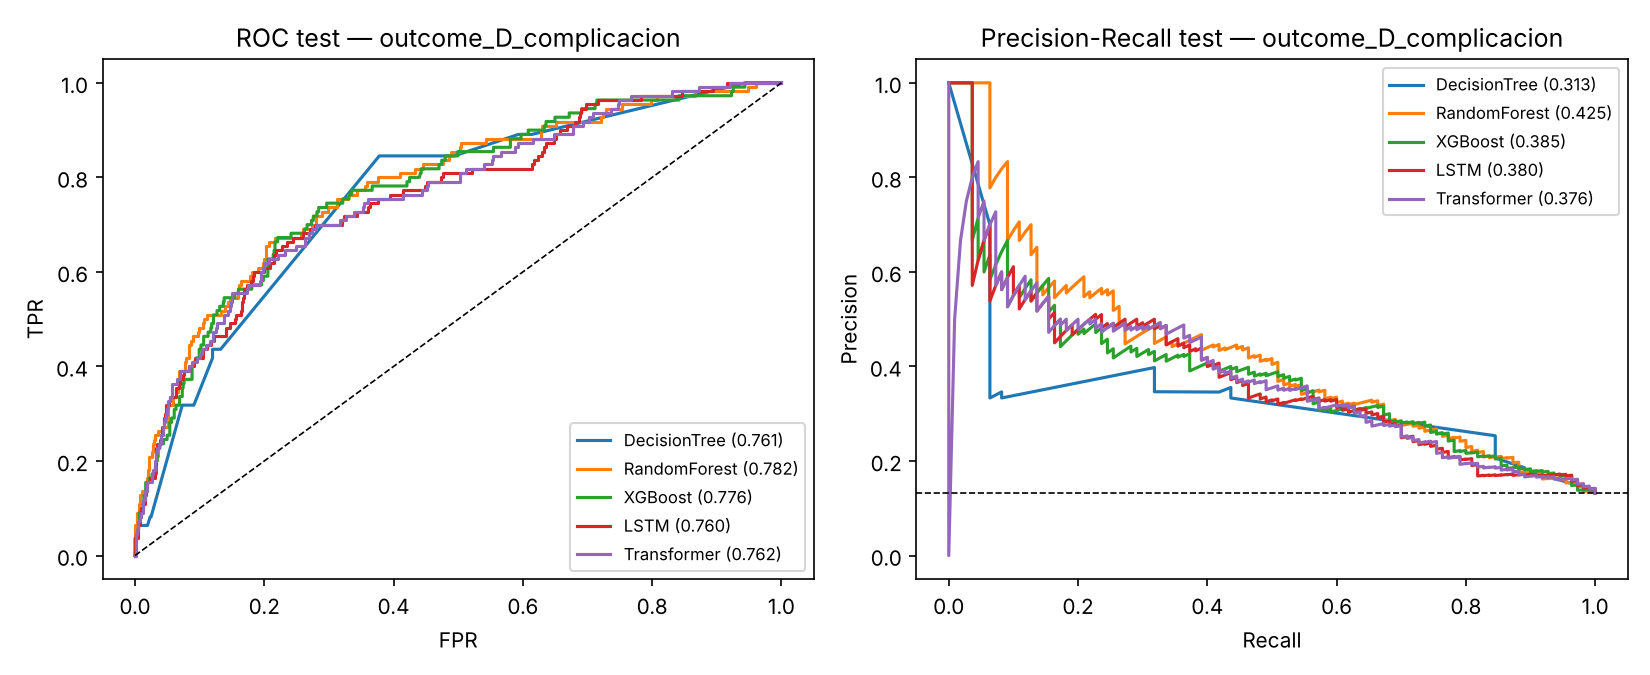
\includegraphics[width=\textwidth]{outcome_D_complicacion_curvas}
\caption{Complementary D: ROC and precision--recall curves for postoperative complication.}
\label{fig:D}
\end{figure}

\subsection{Sensitivity to the Number of Diagnoses}
\label{sec:sens_ndiag}

All the previous results exclude the \code{n\_diag} variable. Table~\ref{tab:ndiag} shows what happens when it is included. In the predictions with signal of their own the effect is mixed and small; in unplanned ICU admission, \code{n\_diag} doubles the AUC-PR and becomes the most important variable (0.21). It is the leakage symptom that was to be expected, since the complication generates diagnoses, and confirms the decision to exclude it. In the test on version 2 of the event log, the static-variable filter of LSTM and Transformer already excluded it unintentionally; in the final version the models are compared with the same information.

\begin{table}[htbp]
\centering
\caption{Sensitivity to \code{n\_diag}: AUC-ROC / AUC-PR with and without the variable.}
\label{tab:ndiag}
\begin{tabular}{lcc}
\toprule
Experiment & Without \code{n\_diag} (main) & With \code{n\_diag} \\
\midrule
Prediction~2 $\cdot$ RF & 0.876 / 0.399 & 0.853 / 0.451 \\
Prediction~2 $\cdot$ XGBoost & 0.846 / 0.280 & 0.755 / 0.353 \\
B $\cdot$ RF & 0.969 / 0.806 & 0.954 / 0.760 \\
C $\cdot$ RF, exit of the operating theater & 0.873 / 0.059 & 0.928 / 0.116 \\
\bottomrule
\end{tabular}
\end{table}

\section{Synthesis and Comparison With the Entropy-Driven Next Activity Prediction Approach}

\subsection{The Three Targets Side by Side}

Figure~\ref{fig:sintesis} shows the main metric of each prediction by model, and Table~\ref{tab:sintesis} gathers the main results of the three outcome-based targets (Predictions~2 and 3 and the complementary analysis D). Together they allow three observations.

\begin{figure}[htbp]
\centering
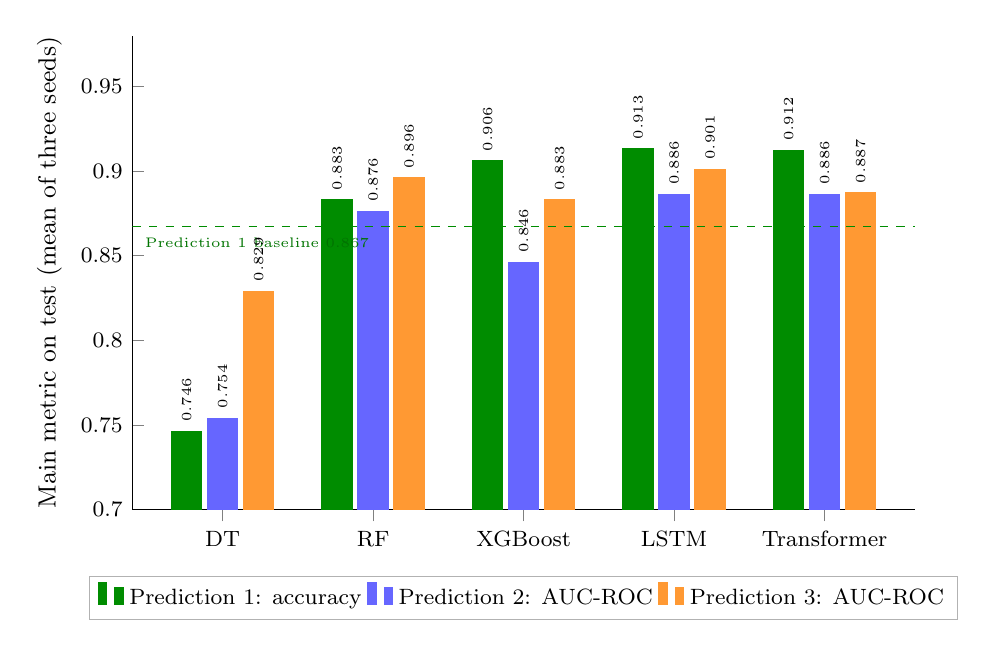
\begin{tikzpicture}
\begin{axis}[
  ybar, width=0.95\textwidth, height=7.6cm, bar width=11pt,
  ymin=0.70, ymax=0.98, xmin=-0.6, xmax=4.6,
  ylabel={Main metric on test (mean of three seeds)}, ylabel style={font=\small},
  xtick={0,1,2,3,4}, xticklabels={DT, RF, XGBoost, LSTM, Transformer},
  tick label style={font=\footnotesize},
  nodes near coords, nodes near coords style={font=\tiny, rotate=90, anchor=west, /pgf/number format/fixed, /pgf/number format/precision=3, /pgf/number format/fixed zerofill},
  axis x line*=bottom, axis y line*=left,
  legend style={at={(0.5,-0.14)}, anchor=north, legend columns=3, font=\footnotesize, draw=black!30}]
\addplot[fill=green!55!black, draw=green!55!black] coordinates {(0,0.746) (1,0.883) (2,0.906) (3,0.913) (4,0.912)};
\addplot[fill=blue!60, draw=blue!60] coordinates {(0,0.754) (1,0.876) (2,0.846) (3,0.886) (4,0.886)};
\addplot[fill=orange!80, draw=orange!80] coordinates {(0,0.829) (1,0.896) (2,0.883) (3,0.901) (4,0.887)};
\legend{Prediction~1: accuracy, Prediction~2: AUC-ROC, Prediction~3: AUC-ROC}
\draw[green!55!black, dashed] (axis cs:-0.6,0.867) -- (axis cs:4.6,0.867);
\node[font=\tiny, green!45!black, anchor=north west] at (axis cs:-0.58,0.866) {Prediction~1 baseline 0.867};
\end{axis}
\end{tikzpicture}
\caption{Main metric of each prediction on test by model: accuracy for Prediction 1 and AUC-ROC for Predictions 2 and 3, mean of three seeds. The dashed line is the most-frequent-transition baseline of Prediction 1.}
\label{fig:sintesis}
\end{figure}

\begin{table}[htbp]
\centering
\caption{Synthesis: AUC-ROC / AUC-PR on test for the three outcome targets.}
\label{tab:sintesis}
\small
\begin{tabular}{lccc}
\toprule
Model & Prediction~2 ICU & Prediction~3 Stay & D Complication \\
 & (8.1\%) & (11.8\%) & (13.2\%) \\
\midrule
DT & 0.754 / 0.205 & 0.829 / 0.416 & 0.761 / 0.313 \\
RF & 0.876 / 0.399 & 0.896 / 0.475 & \textbf{0.781 / 0.422} \\
XGBoost & 0.846 / 0.280 & 0.883 / 0.478 & 0.775 / 0.380 \\
LSTM & \textbf{0.886 / 0.413} & \textbf{0.901 / 0.547} & 0.758 / 0.374 \\
Transformer & \textbf{0.886 / 0.411} & 0.887 / 0.533 & 0.761 / 0.372 \\
\midrule
AUC-PR / prevalence & $\times$5.1 & $\times$4.6 & $\times$3.2 \\
Minimum Brier & 0.081 (RF) & 0.091 (RF) & 0.129 (RF) \\
\bottomrule
\end{tabular}
\end{table}

First, the order of difficulty of the targets is length of stay $<$ ICU admission $<$ complication. The length of stay depends on what is known at admission. ICU admission depends on it only partly, and what is missing is revealed by the surgery. The broad complication includes events that depend on the evolution and on the practice of each service. Second, the winner depends on the signal: with enough signal (Predictions~1, 2 and 3) the sequence models win in ranking, but by a small margin over RF: 3.0 points of accuracy in Prediction~1, 1.0 point of AUC-ROC in Prediction~2 and 0.5 in Prediction~3. With weak signal or few positives (complementary analyses D and C) RF wins. Transformer and LSTM are indistinguishable in Prediction~1 (0.912 versus 0.913) and in Prediction~2 (0.886 for both), and LSTM is 1.4 points ahead in Prediction~3. Third, RF is the best calibrated in the three targets (Brier 0.08--0.13 versus 0.13--0.18 for the deep models), the one that suffers least when the target gets harder and the cheapest (2 s versus 13--40 s). Transformer does not outperform LSTM in any case with traces of one to six events.

\subsection{Comparison with the Protocol of the Entropy-Driven Next Activity Prediction Approach}

Table~\ref{tab:zare_vs} contrasts the experimental protocol of this work with that of the reference paper, based on the parameters it publishes (its Section 4.1 and its Tables 2 and 3).

\begin{table}[htbp]
\centering
\caption{Experimental protocol of the Entropy-Driven Next Activity Prediction Approach versus that of this work.}
\label{tab:zare_vs}
\small
\begin{tabular}{L{2.4cm}L{5.4cm}L{5.4cm}}
\toprule
Parameter & Entropy-Driven Next Activity Prediction Approach & This work \\
\midrule
Predictions & Next-activity prediction only & Next-activity prediction (Prediction~1) and two outcome-based predictions (Predictions~2 and 3) \\
Event logs & Six public ones, from 781 to 150,370 cases & One built for this work, 1,475 cases \\
Prefixes & Complete history padded to the longest trace & $k$-prefixes from 1 to 6; with a median of five they cover almost the whole history \\
Split & 80 / 20 training--validation, `separate' test set without details & Temporal by case, 64 / 16 / 20 \\
Repetitions & No seeds or standard deviations reported & Three seeds, mean $\pm$ standard deviation \\
Imbalance & Subsampling, only for the Transformer on Road Traffic Fine & Class weights in the models \\
Metrics & Accuracy and entropy of the confusion matrix & AUC-ROC, AUC-PR, F1-score, Brier, AUC per prefix; accuracy and macro F1-score \\
Recurrent model & CNN-BiLSTM: convolutions 64/128/256, BiLSTM 400, 300 epochs, batch 32 & LSTM 64 units, embedding 16, up to 80 epochs, batch 64 \\
Transformer & DAW-Transformer: embedding 256, 8 heads, FFN 256, batch 2, 50 epochs & $d=32$, 4 heads, 2 layers, FFN 64, dropout 0.1 \\
Tree-based models & Hyperparameters not published & DT depth 6; RF 300 trees; XGBoost 400 trees with early stopping \\
\bottomrule
\end{tabular}
\end{table}

Three differences deserve comment. The deep models of this work are much smaller than those of the paper ($d=32$ versus 256; 64 units versus 400). This is consistent with the size of the event log (four to six thousand prefixes versus tens or hundreds of thousands of events), but it leaves open the question of whether a larger model would change the conclusion. The paper uses the complete history of the case and criticizes fixed-length windows; in this event log, with a median of five events, six prefixes are practically the whole history, and therefore the difference is only nominal. Moreover, the protocol of this work is stricter in three respects (temporal split, repetition with seeds and imbalance-sensitive metrics), which makes it possible to trust that differences of half a point between models are not noise.

The conclusion, on the other hand, is shared: on a medium-entropy event log, the advantage of the deep models over the classical ensemble is small. What the paper shows with six public event logs on next-activity prediction is reproduced here with a clinical event log built for this work and on three predictions.
